\chapter{Prototypische Umsetzung}
\label{chap:umsetzung}
Dieses Kapitel dokumentiert die Umsetzung des in
Kapitel~\ref{chap:konzept} beschriebenen Konzepts. Da eine
vollständige Wiedergabe des Quellcodes weder möglich noch
aufschlussreich wäre, folgt die Auswahl der Beispiele zwei
Gesichtspunkten: Sie zeigen entweder ein Muster, das an mehreren
Stellen der Anwendung wiederkehrt, oder eine Entscheidung, die sich
aus dem Code allein nicht erschließt. Die eingesetzten Werkzeuge
sind in Abschnitt~\ref{sec:technologieauswahl} beschrieben, die
Ordnerstruktur in Abschnitt~\ref{subsec:komponentenarchitektur}.
\section{Netzwerkkommunikation und Server-State}
\label{sec:impl_netzwerk}
 
Dieser Abschnitt beschreibt die konkrete Umsetzung des in
Abschnitt~\ref{subsec:netzwerk_konzept} vorgestellten
Drei-Schichten-Modells: einer zentralen \acs{HTTP}-Infrastruktur auf
Basis von Axios, einer feature-spezifischen \acs{API}-Schicht sowie
Query-Hooks auf Basis von TanStack Query, die den Verbindungszustand
für die aufrufenden Komponenten bereitstellen.
 
\subsection{HTTP-Client als Infrastruktur}
\label{subsec:impl_httpclient}
 
Die technische Infrastruktur der Netzwerkkommunikation wird durch
eine einzige, projektweit wiederverwendete Axios-Instanz
bereitgestellt \cite{axios_docs}. Listing~\ref{lst:http-client-infra}
zeigt deren vollständige Konfiguration. Die Instanz wird mit einer
festen Basis-Adresse sowie einheitlichen Standard-Headern
initialisiert; die Basis-Adresse lässt sich über eine
Umgebungsvariable überschreiben, sodass zwischen verschiedenen
Backend-Umgebungen gewechselt werden kann, ohne den Quellcode
anzupassen.
 
\begin{lstlisting}[caption={Zentrale Axios-Instanz mit
Request-Interceptor (http-client.ts)},
label={lst:http-client-infra}]
export const httpClient = axios.create({
  baseURL: resolveApiBaseUrl(),
  headers: {
    Accept: 'application/json',
    'Accept-Language': 'en',
    'Content-Type': 'application/json',
  },
})
 
httpClient.interceptors.request.use((config) => {
  const token = getAuthToken()
 
  if (token) {
    config.headers.Authorization = `Bearer ${token}`
  }
 
  return config
})
\end{lstlisting}
 
Über den Request-Interceptor wird der Authentifizierungstoken
automatisch an jede ausgehende Anfrage angehängt, sofern eine
gültige Sitzung vorliegt. Dadurch muss sich keine der
nachfolgend beschriebenen Feature-API-Funktionen selbst um die
Token-Übermittlung kümmern.
 
\subsection{Feature-API-Schicht}
\label{subsec:impl_featureapi}
 
Jeder Funktionsbereich definiert eigene \acs{API}-Funktionen, die
festlegen, welcher Endpunkt mit welcher \acs{HTTP}-Methode und welchen
Parametern angefragt wird. Diese Funktionen greifen ausschließlich
auf den in Abschnitt~\ref{subsec:impl_httpclient} beschriebenen
\texttt{httpClient} zurück und sind selbst frei von
Infrastruktur-Details. Listing~\ref{lst:feature-api-getme} zeigt
dies am Beispiel der Funktion \texttt{getMe()} aus dem
Account-Feature, die um optionale Parameter für die Einbindung einer
Zusammenfassung sowie eine Begrenzung der zurückgegebenen
Einträge ergänzt ist.
 
\begin{lstlisting}[caption={Feature-API-Funktion getMe
(account-api.ts)}, label={lst:feature-api-getme}]
export async function getMe(includeSummary = false, limit?: number) {
  const params = new URLSearchParams()
 
  if (includeSummary) {
    params.set('include', 'summary')
  }
 
  if (typeof limit === 'number') {
    params.set('limit', String(limit))
  }
 
  const queryString = params.toString()
  const path = queryString
    ? `${accountEndpoints.me}?${queryString}`
    : accountEndpoints.me
 
  const response = await httpClient.get<ApiSuccessResponse<MeResult>>(path)
 
  return response.data
}
\end{lstlisting}
 
Die Funktion baut die Query-Parameter abhängig von den übergebenen
Argumenten zusammen und gibt ausschließlich die Nutzdaten der
Antwort zurück. Sie enthält selbst keine Logik zur Behandlung von
Lade- oder Fehlerzuständen; diese Aufgabe übernimmt die in
Abschnitt~\ref{subsec:impl_tanstackquery} beschriebene Query-Hook-Schicht.
 
\subsection{Server-State mit TanStack Query}
\label{subsec:impl_tanstackquery}
 
Die oberste Schicht bilden Query-Hooks, die eine Feature-API-Funktion
mithilfe von TanStack Query kapseln und den aufrufenden Komponenten
den Zustand der Verbindung bereitstellen \cite{tanstack_query_docs}.
Listing~\ref{lst:use-me-query} zeigt den Hook
\texttt{useMeQuery}, der die zuvor beschriebene Funktion
\texttt{getMe()} verwendet.
 
\begin{lstlisting}[caption={Query-Hook useMeQuery
(use-me-query.ts)}, label={lst:use-me-query}]
export function useMeQuery(includeSummary = false, limit?: number, enabled = true) {
  return useQuery({
    queryKey: ['me', { includeSummary, limit }],
    queryFn: () => getMe(includeSummary, limit),
    enabled,
  })
}
\end{lstlisting}
 
Der \texttt{queryKey} setzt sich, wie in
Abschnitt~\ref{subsec:netzwerk_konzept} beschrieben, aus einer
festen Bezeichnung und den übergebenen Parametern zusammen und
identifiziert die Anfrage eindeutig im projektweiten Cache. Der
\texttt{enabled}-Parameter erlaubt es zusätzlich, die Ausführung
der Anfrage an eine Bedingung zu knüpfen, etwa das Vorhandensein
einer gültigen Sitzung.
 
Der Rückgabewert des Hooks stellt der aufrufenden Komponente die
Felder \texttt{data}, \texttt{isLoading} und \texttt{isError} zur
Verfügung, über die sich Ladeindikatoren und Fehlermeldungen
umsetzen lassen. In der Kontoübersicht wird dieses Muster
vereinfacht eingesetzt: Anstelle einer expliziten Auswertung von
\texttt{isLoading} und \texttt{isError} greift die Komponente auf
einen Fallback auf die bereits im Client gespeicherte Sitzung
zurück, sodass dem Nutzer zumindest der Benutzername angezeigt
werden kann, selbst wenn die Anfrage an das Backend noch nicht
abgeschlossen ist oder fehlschlägt. Für Ansichten ohne einen
solchen Fallback ist hingegen eine explizite Behandlung der von
TanStack Query bereitgestellten Zustände erforderlich.
 
Die Query-Hooks greifen dabei auf einen einmalig erzeugten,
zentralen Cache zurück, der über die gesamte Anwendung hinweg
geteilt wird und beim Anwendungsstart über einen Provider
bereitgestellt wird. Über die Zwischenspeicherung bereits
abgerufener Daten hinaus bietet TanStack Query den Mechanismus der
gezielten Invalidierung von Cache-Einträgen; dieser bildet die
alleinige, projektweit einheitliche Grundlage für die Aktualität
zwischengespeicherter Daten, anstelle einer zusätzlichen
Konfiguration fester Gültigkeitsdauern. Dieses Muster aus Query
Key, Cache und einheitlichen Verbindungszuständen kommt bei
sämtlichen weiteren Datenabrufen der Anwendung in gleicher Form
zum Einsatz und wird in den folgenden Abschnitten jeweils nur
noch kurz referenziert.
\section{Mehrsprachigkeit der Oberfläche}
\label{sec:impl_i18n}
 
Die Umsetzung des in
Abschnitt~\ref{subsec:mehrsprachigkeit_konzept} beschriebenen
Konzepts stützt sich auf \textit{i18next} mit der React-Anbindung
\textit{react-i18next} \cite{i18next_docs}. Die Oberflächentexte
liegen in zwei Modulen, je eines für Deutsch und Englisch; beide
enthalten dieselben Schlüssel und unterscheiden sich allein in den
Werten. Die Schlüssel sind nicht alphabetisch, sondern nach ihrem
Verwendungsbereich gruppiert -- etwa \texttt{header},
\texttt{cart} oder \texttt{checkout} --, wobei ein Bereich
\texttt{common} die mehrfach verwendeten Texte aufnimmt. Dieselbe
Bezeichnung kann dadurch in verschiedenen Bereichen einen eigenen
Wert tragen.
 
\begin{lstlisting}[caption={Auszug aus der deutschen Ressourcendatei (de.ts)}, label={lst:i18n-messages}]
const de = {
  common: {
    cart: 'Warenkorb',
    noDescriptionYet: 'Noch keine Beschreibung.',
  },
  catalog: {
    bySeller: 'von {{name}}',
  },
  checkout: {
    successTitle: 'Checkout erfolgreich',
    paymentConfirmed: 'Zahlung bestaetigt',
  },
}
\end{lstlisting}
 
Der Eintrag \texttt{bySeller} zeigt die Behandlung veränderlicher
Bestandteile: Der Platzhalter wird beim Anzeigen ersetzt, sodass der
Satzbau in der Ressourcendatei verbleibt und nicht im Quelltext
zusammengesetzt wird -- was nötig ist, da die Stellung eines
eingesetzten Wortes von Sprache zu Sprache verschieden ist.
 
Die Konfiguration erfolgt an einer Stelle und wird beim Start noch
vor der ersten Darstellung ausgeführt. Sie legt die Ressourcen, die
Rückfallsprache und die Reihenfolge fest, in der die Sprache
ermittelt wird: zunächst der gespeicherte Wert, andernfalls die
Spracheinstellung des Browsers. Die Wahl wird im
\texttt{localStorage} abgelegt, derselben Ablage wie die Sitzung
(vgl. Abschnitt~\ref{subsec:impl_token_session}), und ist in einem
eigenen Hook gekapselt; der Umschalter greift ausschließlich darauf
zu und kennt weder die Bibliothek noch die Art der Speicherung.
 
Die Inhalte aus dem Backend werden dagegen nicht übersetzt, sondern
angefordert: Der in Abschnitt~\ref{subsec:impl_httpclient}
beschriebene zentrale \acs{HTTP}-Client führt bei jeder Anfrage einen
Header mit der gewählten Sprache mit. Der Wert wird im Interceptor
gesetzt und nicht bei der Erzeugung der Instanz, da er sonst auf dem
Stand des Anwendungsstarts bliebe. Eine einzige Stelle genügt damit,
um die Sprachwahl auf sämtliche Inhalte wirken zu lassen.
 
Sichtbar wird dies gegenwärtig gleichwohl nicht: Die
Erfassungsformulare sehen Englisch und Arabisch vor (vgl.
Abschnitt~\ref{subsec:impl_dienstleistungsverwaltung}), sodass keine
deutsche Fassung der Inhalte entsteht und das Backend auf die
deutsche Anforderung mit der englischen antwortet. Die Übertragung
der Sprachwahl ist im Frontend somit vollständig umgesetzt, wirkt
sich auf die Inhalte jedoch erst aus, sobald das Datenmodell eine
deutsche Fassung vorsieht.
\section{Authentifizierung und Onboarding}
\label{sec:impl_auth}

\subsection{Registrierung und Login}
\label{subsec:impl_registrierung_login}
 
Entsprechend dem Konzept aus
Abschnitt~\ref{subsec:auth-onboarding} ist die Registrierung als
eigene Seite umgesetzt, der Login als Dialog. Dieser überlagert die
aufrufende Seite, ohne sie zu ersetzen, sodass der Nutzer nach der
Anmeldung ohne Umweg an die Stelle zurückkehrt, an der er sich befand.
 
\begin{figure}[H]
\centering
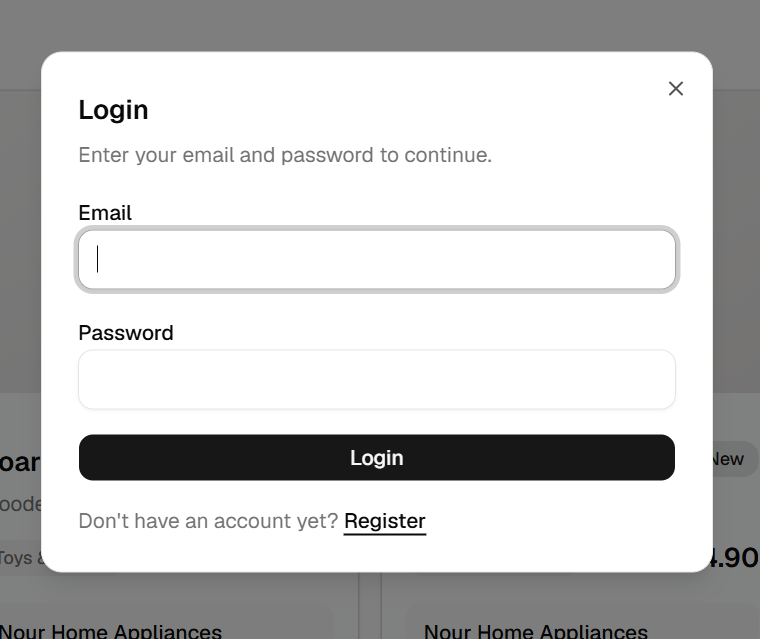
\includegraphics[width=0.7\textwidth]{Bilder/screenshot_login_dialog.png}
\caption{Login-Dialog}
\label{fig:login_dialog}
\end{figure}
 
Beide Formulare werden über \texttt{react-hook-form} in Verbindung
mit einem Zod-Schema validiert (vgl.
Abschnitt~\ref{subsec:formulare-validierung}). Das Schema der
Registrierung prüft dabei nicht nur einzelne Felder, sondern auch
deren Verhältnis zueinander.
 
\begin{lstlisting}[caption={Validierungsschema der Registrierung (register-schema.ts)}, label={lst:register-schema}]
export const registerSchema = z
  .object({
    name: z
      .string()
      .trim()
      .min(1, 'Name is required.')
      .max(255, 'Name must be 255 characters or fewer.'),
    age: z.preprocess(
      (value) =>
        value === '' || value === undefined || Number.isNaN(value) ? null : value,
      z
        .number({ error: 'Enter a valid age.' })
        .int()
        .min(12, 'Age must be at least 12.')
        .max(100, 'Age must be 100 or less.')
        .nullable(),
    ),
    email: z
      .string()
      .trim()
      .min(1, 'Email is required.')
      .email('Enter a valid email address.'),
    phone: z.preprocess(emptyToUndefined, z.string().optional()),
    password: z.string().min(6, 'Password must be at least 6 characters.'),
    password_confirmation: z.string().min(1, 'Please confirm your password.'),
  })
  .superRefine((values, context) => {
    if (values.password !== values.password_confirmation) {
      context.addIssue({
        code: 'custom',
        message: 'Passwords do not match.',
        path: ['password_confirmation'],
      })
    }
  })
\end{lstlisting}
 
Die einzelnen Feldregeln lassen sich unabhängig voneinander prüfen.
Die Übereinstimmung von Passwort und Bestätigung dagegen nicht, da
sie zwei Werte zugleich betrifft; sie wird deshalb über
\texttt{superRefine} auf der Ebene des gesamten Objekts geprüft und
über die Angabe eines Pfades dem Bestätigungsfeld zugeordnet. Eine
eigene Längenregel benötigt das Bestätigungsfeld dadurch nicht: Da
es dem Passwort entsprechen muss und dieses mindestens sechs Zeichen
umfasst, ergibt sich seine Länge aus der Übereinstimmung.
 
Die beiden freiwilligen Felder werden vor der Prüfung aufbereitet.
Beim Telefonfeld ersetzt eine Hilfsfunktion eine leer gebliebene
Eingabe durch \texttt{undefined}, beim Altersfeld durch
\texttt{null}, sodass ein nicht ausgefülltes Feld nicht als leerer
Text an das Backend gelangt. Bei den Pflichtfeldern unterbleibt
diese Aufbereitung, und es genügt \texttt{trim}: Dort ist eine leere
Eingabe gerade der Fehlerfall und darf nicht in einen fehlenden Wert
umgedeutet werden, weil die zugehörige Regel sonst nicht mehr
greifen könnte.
 
\begin{figure}[H]
\centering
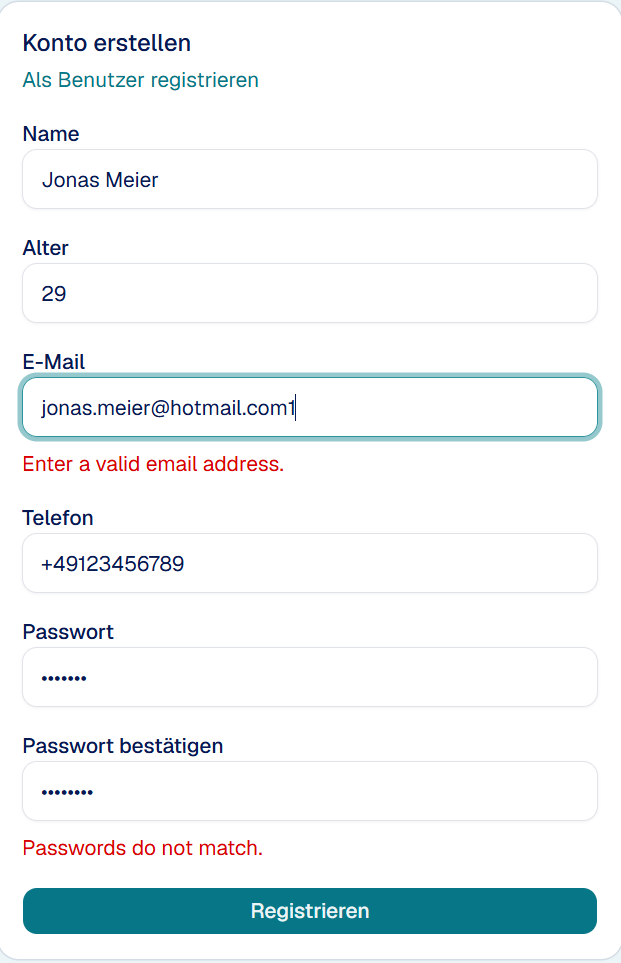
\includegraphics[width=0.55\textwidth]{Bilder/screenshot_registrierung_fehler.png}
\caption{Registrierungsformular mit einem Formatfehler im
E-Mail-Feld und einer feldübergreifenden Abweichung zwischen Passwort
und Bestätigung}
\label{fig:registrierung_fehler}
\end{figure}
 
Die Meldungen stehen unmittelbar unter dem betroffenen Feld,
benennen die verletzte Regel und bleiben stehen, bis die Eingabe
korrigiert ist; die übrigen Eingaben bleiben erhalten, sodass ein
fehlgeschlagener Versuch nicht zum erneuten Ausfüllen des gesamten
Formulars zwingt (vgl.
Abschnitt~\ref{subsec:gestaltungsprinzipien}).
 
Nicht alle Prüfungen können im Frontend stattfinden: Ob eine
E-Mail-Adresse bereits vergeben ist oder ein Passwort dem
hinterlegten entspricht, kann nur das Backend beantworten.
Serverseitig gemeldete Fehler werden deshalb demselben Feld
zugeordnet und in derselben Form dargestellt wie clientseitige;
nicht zuordenbare Fehler erscheinen als allgemeine Meldung über dem
Formular.
 
Verläuft die Anfrage erfolgreich, wird die Sitzung im
Authentifizierungszustand gespeichert; beim Login schließt sich der
Dialog, bei der Registrierung erfolgt eine Weiterleitung auf die
Startseite.

\subsection{Token-Verwaltung und Session-Handling}
\label{subsec:impl_token_session}
Die Session der Anwendung ist als eigenes Modell definiert, das
Zugriffstoken, Nutzerdaten und die zugewiesenen Rollen als Liste
enthält, da ein Nutzer mehrere Rollen gleichzeitig besitzen kann. Sie
wird über einen zentralen Zustand-Store reaktiv bereitgestellt und im
\texttt{localStorage} des Browsers gespeichert, um den Anmeldestatus
über Neuladen und erneute Besuche hinweg zu erhalten.
Listing~\ref{lst:auth-store-state} zeigt die Struktur dieses Stores
sowie dessen Erzeugung über die \texttt{create}-Funktion der
Bibliothek Zustand.
 
\begin{lstlisting}[caption={Struktur und Erzeugung des Auth-Stores (auth-store.ts)}, label={lst:auth-store-state}]
import { create } from 'zustand'
 
interface AuthStoreState {
  session: AuthSession | null
  isAuthenticated: boolean
  isBootstrapping: boolean
  setSession: (session: AuthSession) => void
  setBootstrapping: (isBootstrapping: boolean) => void
  syncVerifiedUser: (user: User) => void
  clearSession: () => void
}
 
export const useAuthStore = create<AuthStoreState>((set, get) => ({
  // ...
}))
\end{lstlisting}
 
Ein gespeicherter Token wird nicht ungeprüft als gültig angenommen:
Eine Bootstrap-Komponente validiert ihn aktiv beim Backend über
\texttt{useMeQuery} (vgl.
Abschnitt~\ref{subsec:impl_tanstackquery}). Liefert diese Anfrage
einen Fehler, gilt der Token als ungültig und die Session wird über
den Store verworfen; liefert sie hingegen aktualisierte Nutzerdaten,
werden diese im Store synchronisiert, sodass lokal gespeicherte und
serverseitig bestätigte Daten konsistent bleiben. Liegt noch keine
Antwort vor, wird zunächst die lokal gespeicherte Session verwendet,
damit die Oberfläche sofort angezeigt werden kann. Auf dieser
Grundlage entscheidet eine geschützte Routenkomponente, ob der
Anmeldestatus noch ermittelt wird, der Nutzer zur Startseite
weitergeleitet oder der geschützte Inhalt angezeigt wird.

\subsection{Rollen-Upgrade-Antrag}
\label{subsec:impl_rollen_upgrade}

Wie in Abschnitt~\ref{subsec:auth-onboarding} beschrieben, kann
ein Nutzer über die Kontoübersicht einen Antrag auf die Rolle
	extit{Seller} oder 	extit{ServiceProvider} stellen. Zusätzlich zu den Basisdaten
werden dabei projektspezifische Angaben wie Name und Kontaktdaten
des Geschäfts sowie ein Nachweisdokument erfasst, anhand derer ein
Administrator über den Antrag entscheidet. Bis zur Entscheidung
bleibt der Nutzer uneingeschränkt in seiner Rolle als 	extit{Customer}
aktiv; nach einer Genehmigung stehen ihm zusätzliche,
rollenspezifische Seiten zur Verfügung.

% TODO (Roudy): Hier Screenshot der Kontouebersicht vor und nach
% der Genehmigung nebeneinander einfuegen (vgl. Meeting vom
% 12.07.2026), kein Code, kein Diagramm.
\section{Katalog und Produktseiten}
\label{sec:impl_katalog}

\subsection{Produktlisting: Karten, Paginierung}
\label{subsec:impl_produktlisting}

Dieser Abschnitt beschreibt die Umsetzung der in
Abschnitt~\ref{subsec:katalog_konzept} vorgestellten Startseite
sowie das wiederverwendbare Kartenprinzip, das dort zum Einsatz
kommt. Die Startseite ruft ihre Daten über eine einzelne, an den
Endpunkt \texttt{/api/home} gerichtete Anfrage ab, die Produkte
und Dienstleistungen gemeinsam liefert. Der Aufbau der
Anfragefunktion und des zugehörigen Query-Hooks folgt dabei
demselben Prinzip, das bereits in
Abschnitt~\ref{sec:impl_netzwerk} eingeführt wurde. Während des
Ladens wird ein Platzhalter-Raster angezeigt, im Fehlerfall eine
Fehlermeldung; im Unterschied zur Kontoübersicht (vgl.
Abschnitt~\ref{subsec:impl_tanstackquery}) steht hier keine
lokal gespeicherte Alternative zur Verfügung, sodass diese
Zustände explizit behandelt werden.

Sowohl der Produkt- als auch der Dienstleistungsbereich der
Startseite nutzen dieselbe wiederverwendbare
Vorschau-Komponente, die Titel, Leer-Zustand-Nachricht und den
eigentlichen Karteninhalt entgegennimmt. Jedes Produkt wird über
eine Karte dargestellt, die den vom Backend gelieferten,
unvollständigen Bildpfad um die Basis-Adresse ergänzt, den Preis
über die integrierte \texttt{Intl.NumberFormat}-Schnittstelle
formatiert und bei kürzlich hinzugefügten Produkten eine
entsprechende Kennzeichnung anzeigt.

Auf der Katalogseite für Produkte lassen sich die angezeigten
Einträge zusätzlich nach Kategorie filtern und seitenweise
durchblättern; Seite und Kategorie werden als Suchparameter in
der \acs{URL} abgebildet, sodass sich ein bestimmter Ausschnitt des
Katalogs verlinken lässt. Da diese Parameter Teil des Query Keys
sind (vgl. Abschnitt~\ref{subsec:impl_tanstackquery}), führt
sowohl ein Seitenwechsel als auch eine geänderte Kategorie zu
einer neuen Anfrage an das Backend.

\subsection{Produktdetailseite \& Dienstleistungsdetailseite}
\label{subsec:impl_produktdetail}

Der Aufruf einer Produktkarte führt, wie in
Abschnitt~\ref{subsec:katalog_konzept} beschrieben, auf die
zugehörige Detailseite; die Produkt-ID wird dabei als validierter
Routenparameter übergeben (vgl.
Abschnitt~\ref{subsec:routing-konzept}) und an den zugehörigen
Query-Hook weitergereicht. Die Seite unterscheidet vier
Zustände: eine ungültige Produkt-ID, den Ladezustand, einen
Fehler bei der Anfrage sowie den Fall, dass kein Produkt zu der
angefragten ID existiert. Liegen die Produktdaten vor, werden sie
in einer Bildergalerie, die auf dieselbe Bildpfad-Auflösung
zurückgreift wie die Produktkarte, sowie einer Übersicht mit
Preis, Kategorie und Verkäuferinformationen dargestellt.

% ----------------------------------------------------------------
% TODO (Roudy): Screenshot der Startseite mit den
% Vorschau-Karten (Produkte und Dienstleistungen,
% inkl. "New"-Kennzeichnung).

% TODO (Roudy): Screenshot der Produkt-Katalogseite mit
% Kategoriefilter und Paginierung (Seite/Kategorie in der URL
% sichtbar, z. B. /products?page=2&category=3).

% ----------------------------------------------------------------
\subsection{Terminauswahl auf der Dienstleistungsseite}
\label{subsec:impl_terminauswahl}
 
Die in Abschnitt~\ref{subsec:buchung_konzept} beschriebene Auswahl
ist als eigenständige, wiederverwendbare Komponente umgesetzt und auf
der Dienstleistungs-Detailseite eingebunden. Sie durchläuft drei
Zustände.
 
Im Ausgangszustand zeigt sie einen Monatskalender und die Zeitzone
des Anbieters. Welche Zeitfenster ein Tag enthält, ergibt sich erst
aus der Antwort des Backends; die Schaltfläche zur Übernahme in den
Warenkorb bleibt zunächst deaktiviert. Jeder Tag ist anwählbar, auch
ein solcher ohne Arbeitszeit -- an Stelle der Liste erscheint dann
der Hinweis, dass für dieses Datum keine Zeitfenster verfügbar sind
(vgl. Abschnitt~\ref{subsec:verkaeufer_dashboard_konzept}).
 
Mit der Wahl eines Tages wird dessen Zeitfensterliste abgerufen. Die
Fenster werden nach Tageszeit in Vormittag, Nachmittag und Abend
gruppiert; jedes trägt seinen Zeitraum und die verbleibende
Kapazität. Erst mit der Wahl eines Fensters erscheint eine
Zusammenfassung der Buchung, und die Schaltfläche wird aktiv.
 
\begin{figure}[H]
\centering
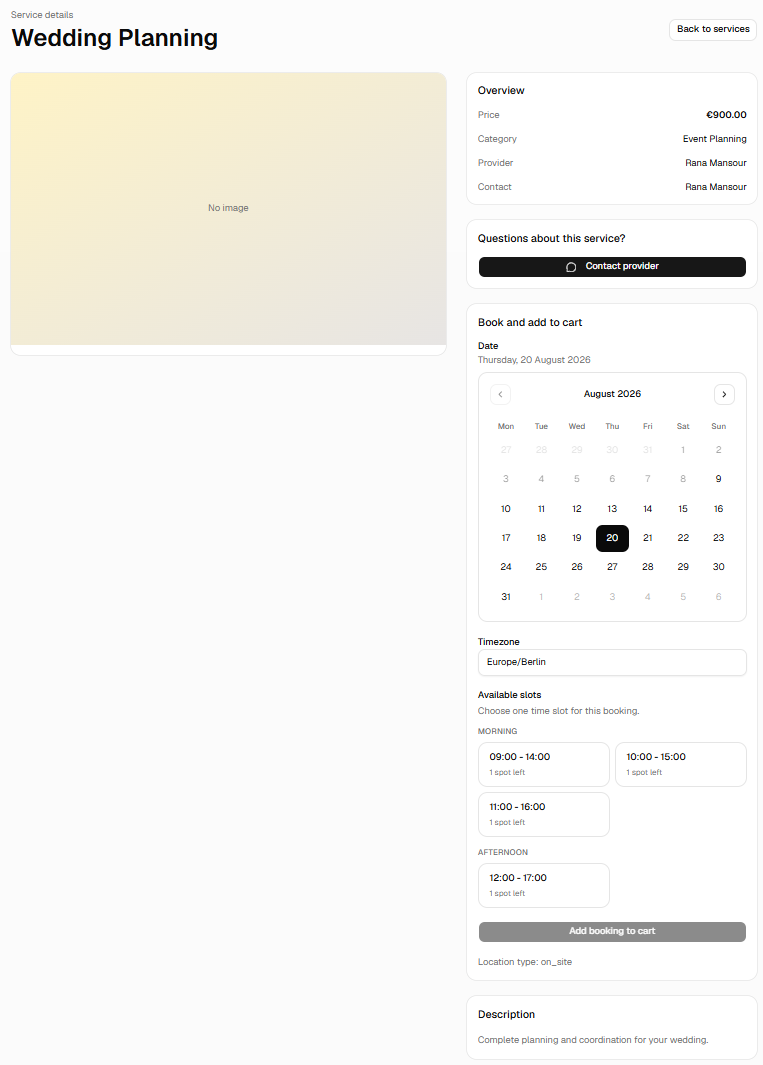
\includegraphics[width=0.60\textwidth]{Bilder/screenshot_buchung_auswahl.png}
\caption{Terminauswahl nach Wahl von Tag und Zeitfenster}
\label{fig:buchung_auswahl}
\end{figure}
 
Am Zeitraster der Fenster ist die Wirkung der Buchungsregeln
ablesbar: Bei einer Dauer von drei Stunden und einem Raster von
dreißig Minuten beginnen aufeinanderfolgende Fenster jeweils eine
halbe Stunde später und überlappen sich damit. Sie schließen einander
nicht aus, solange die Kapazität nicht erschöpft ist.
 
Die Übernahme in den Warenkorb erzeugt eine Position, die neben
Titel, Preis und Kategorie zusätzlich Beginn, Ende, Zeitzone und Ort
der Leistungserbringung trägt (vgl.
Abschnitt~\ref{subsec:impl_warenkorb}).


\section{Warenkorb, Checkout und Zahlung}
\label{sec:impl_checkout}


\subsection{Warenkorb-UI: Produkte und Buchungen kombiniert}
\label{subsec:impl_warenkorb}

Der Warenkorb ist als eigener Zustand-Store umgesetzt, getrennt vom
Auth- und vom \acs{UI}-Store (vgl.
Abschnitt~\ref{subsec:state-management-konzept}). Seine Persistenz
übernimmt die \texttt{persist}-Middleware von Zustand, die den Inhalt
unter dem Schlüssel \texttt{bazario-cart} im \texttt{localStorage}
ablegt \cite{zustand_docs}. Gespeichert wird dabei nicht der gesamte
Store, sondern über \texttt{partialize} nur der übertragbare Teil:
die Positionen, die Währung und die Zuordnung zum Besitzer. Die
abgeleiteten Funktionen für Zwischensumme und Positionszahl bleiben
ausgeschlossen, da sie sich aus den Positionen jederzeit neu
berechnen lassen.
 
Die beiden Positionstypen werden beim Hinzufügen unterschiedlich
behandelt. Ein Produkt wird über seine Kennung erkannt; ist es
bereits enthalten, erhöht sich lediglich dessen Menge. Eine
Dienstleistungsbuchung besitzt dagegen keine Menge, sondern einen
Termin. Zwei Buchungen gelten deshalb nur dann als dieselbe, wenn
sechs Angaben übereinstimmen: die Dienstleistung, Beginn, Ende,
Zeitzone, die Art des Ortes und dessen nähere Bestimmung. Trifft das
zu, bleibt der Warenkorb unverändert; dieselbe Dienstleistung zu
einem anderen Termin ist dagegen eine eigene Position.
 
Ein dritter Punkt ergibt sich daraus, dass der Warenkorb im Browser
verbleibt und nicht am Konto hängt. Er führt deshalb mit, wem er
gehört, und gleicht diese Zuordnung bei jeder Änderung des
Anmeldestatus ab: Meldet sich ein zuvor nicht angemeldeter Nutzer
an, bleiben seine Positionen erhalten und werden ihm zugeordnet.
Wechselt dagegen der angemeldete Nutzer, wird der Warenkorb geleert.
Andernfalls fände ein Nutzer, der sich am selben Gerät anmeldet, die
Positionen seines Vorgängers vor.
\begin{figure}[H]
\centering
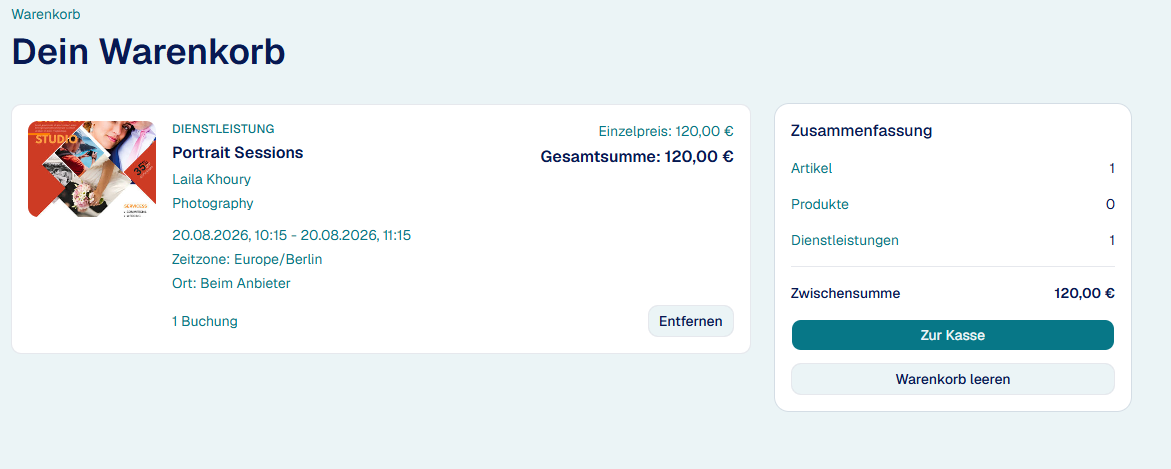
\includegraphics[width=\textwidth]{Bilder/screenshot_warenkorb_buchung.png}
\caption{Dienstleistungsbuchung als Position im Warenkorb}
\label{fig:warenkorb_buchung}
\end{figure}

\subsection{Stripe-Integration im Frontend}
\label{subsec:impl_stripe}
 
Die Umsetzung des in Abschnitt~\ref{subsec:warenkorb_konzept}
beschriebenen Konzepts verteilt sich auf zwei Stellen im Frontend:
das Auslösen des Checkouts im Warenkorb und die Verarbeitung des
Ergebnisses auf den beiden Rückleitungsseiten. Dazwischen liegt eine
Folge von Schritten, an denen Frontend, Backend und Zahlungsdienst
beteiligt sind.
 
\begin{figure}[H]
\centering
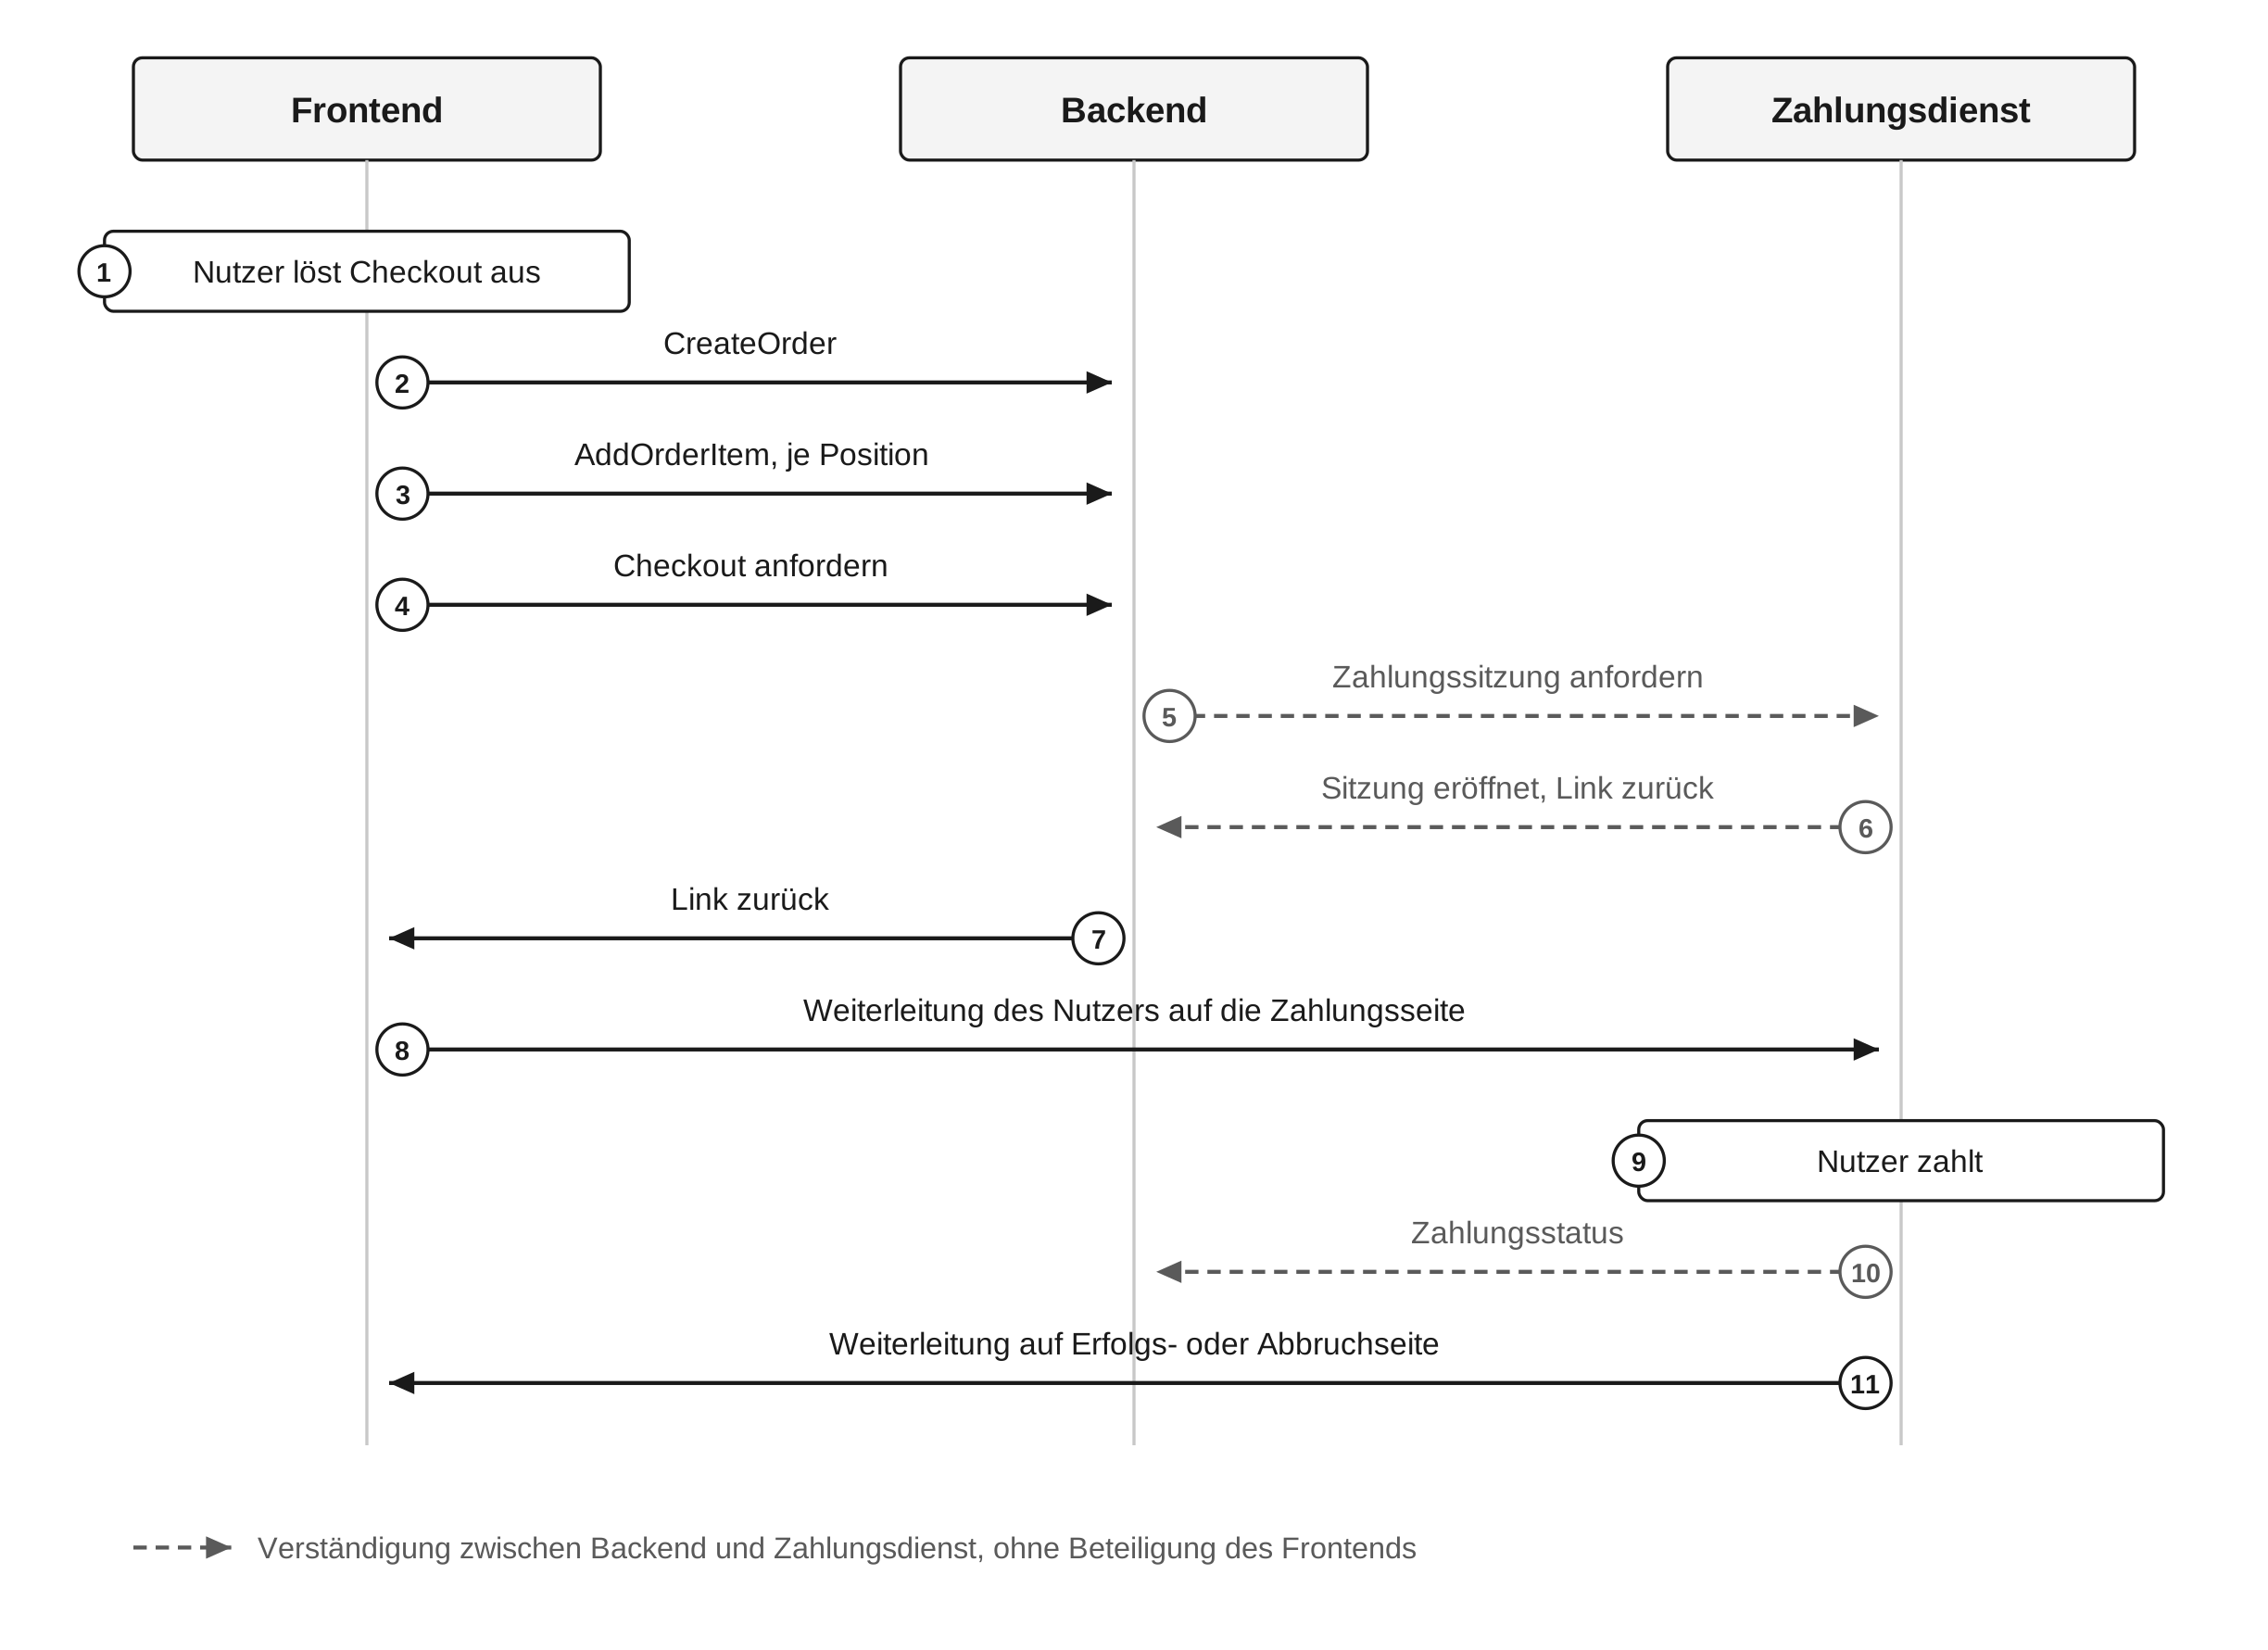
\includegraphics[width=0.8\textwidth]{Bilder/abb_checkout_ablauf.png}
\caption{Ablauf der Zahlung vom Auslösen des Checkouts bis zur
Rückleitung in die Anwendung}
\label{fig:checkout_ablauf}
\end{figure}
 
Vom Frontend gehen dabei nur drei Anfragen aus: das Anlegen des
Auftrags, das Hinzufügen der Positionen und das Anfordern der
Zahlungssitzung. Die Verständigung mit dem Zahlungsdienst erfolgt
vollständig im Backend.
 
Ausgelöst wird der Vorgang über die Schaltfläche in der
Warenkorbübersicht. Ist der Nutzer nicht angemeldet, öffnet die
Funktion über den \acs{UI}-Store den Anmeldedialog und bricht ab; der
Warenkorb bleibt dabei unverändert. Andernfalls läuft die
Checkout-Operation an, die als Mutation umgesetzt ist, da sie den
Datenbestand auf dem Server verändert (vgl.
Abschnitt~\ref{subsec:impl_tanstackquery}). Sie durchläuft drei
Schritte: Zunächst wird über die Feature-\acs{API} ein Auftrag
angelegt, dessen Kennung das Backend zurückgibt. Anschließend wird
für jede Position des Warenkorbs eine weitere Anfrage gestellt, die
sie diesem Auftrag zuordnet. Zuletzt wird die Zahlungssitzung
angefordert; das Backend liefert die Adresse der Zahlungsseite
zurück, auf die das Frontend den Browser weiterleitet.
 
\begin{figure}[H]
\centering
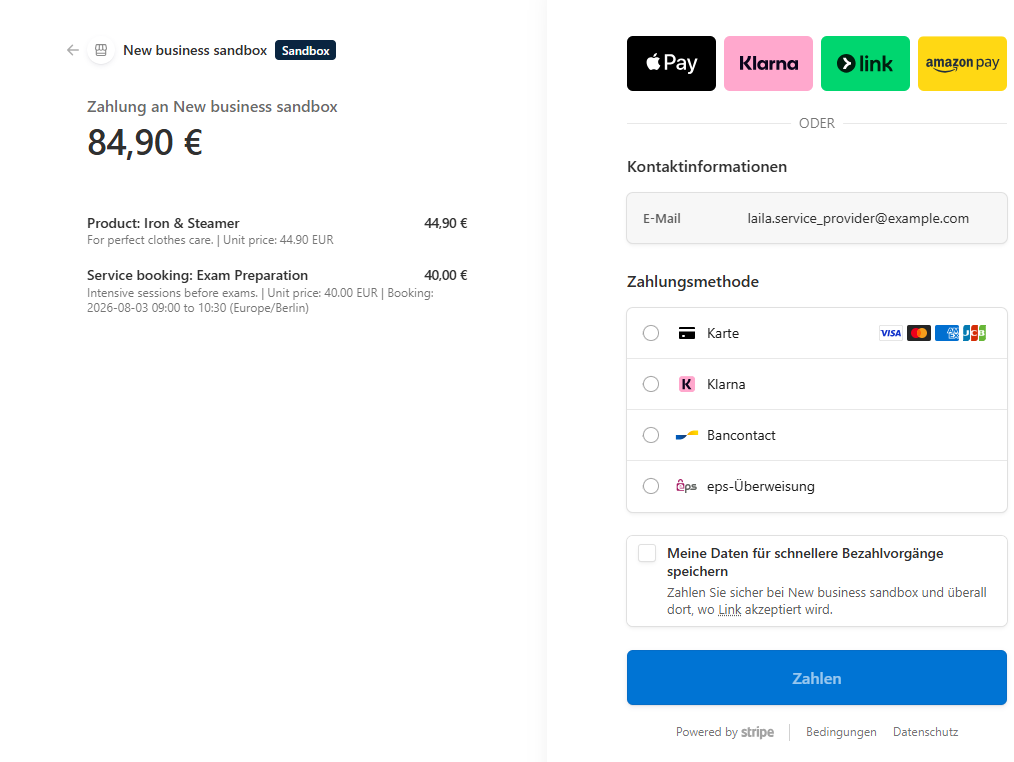
\includegraphics[width=0.7\textwidth]{Bilder/screenshot_stripe_zahlungsseite.png}
\caption{Von Stripe bereitgestellte Zahlungsseite, auf die das
Frontend nach dem Auslösen des Checkouts weiterleitet}
\label{fig:stripe_zahlungsseite}
\end{figure}
 
Die Aufbereitung der einzelnen Position ist in eine eigene Funktion
ausgelagert, da sich die zu übertragenden Angaben je nach
Positionstyp unterscheiden: Für ein Produkt genügen Kennung und
Menge, während eine Dienstleistungsbuchung zusätzlich den gewählten
Termin enthält. Die Fallunterscheidung liegt damit nicht in der
Mutation, die dadurch auf ihre drei Schritte beschränkt bleibt.
 
Nach Abschluss der Zahlung führt der Zahlungsdienst den Nutzer auf
eine der beiden Rückleitungsseiten zurück. Die Erfolgsseite ruft die
Auftragsdaten ab und zeigt Auftragsnummer, Status und Betrag an;
darunter bietet sie zwei Wege in die Übersichten an, getrennt nach
Bestellungen und Buchungen, da ein Auftrag beide Positionstypen
enthalten kann (vgl.
Abschnitt~\ref{subsec:gestaltungsprinzipien}).
 
\begin{figure}[H]
\centering
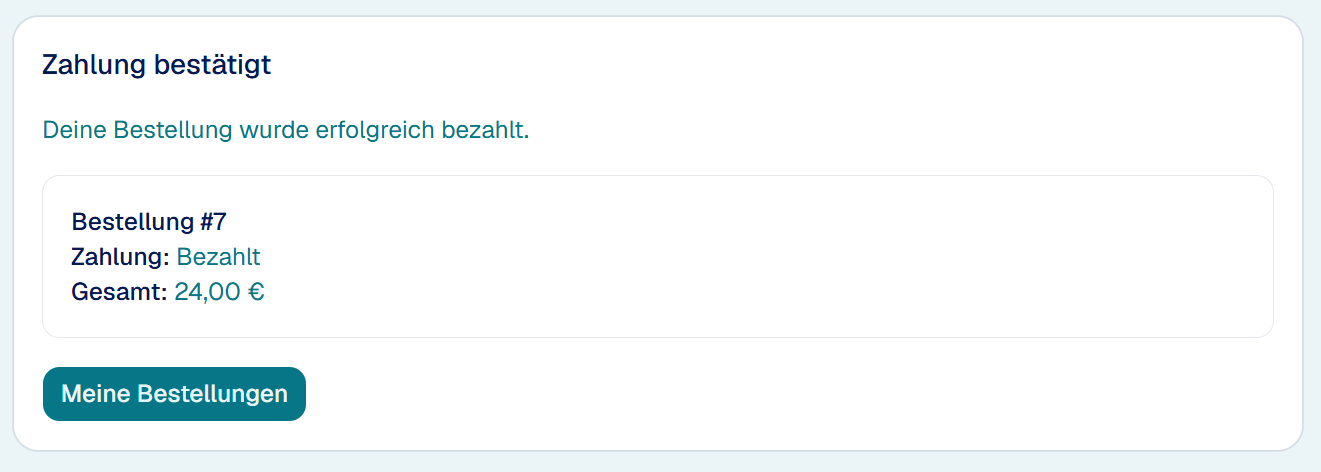
\includegraphics[width=0.85\textwidth]{Bilder/screenshot_checkout_success.png}
\caption{Bestätigungsseite nach erfolgreicher Zahlung}
\label{fig:checkout_success}
\end{figure}
 
Vor der Darstellung führt die Seite eine Folge von Nebenwirkungen
aus, die in einem Effekt gekapselt sind. Der Effekt prüft zunächst,
ob die Zahlung tatsächlich erfolgt ist, und bricht andernfalls ab.
Erst danach wird der Warenkorb geleert -- nicht schon beim Auslösen
des Checkouts, da die Zahlung bis zuletzt scheitern oder abgebrochen
werden kann.
 
Zusätzlich sichert eine Referenz ab, dass der Effekt nur einmal
ausgeführt wird. Ohne diese Sperre könnte ein erneutes Rendern den
Warenkorb ein zweites Mal leeren und die Invalidierung wiederholen,
obwohl derselbe Zahlungsvorgang zugrunde liegt. Eine Referenz eignet
sich dafür, weil ihre Änderung im Gegensatz zu einem Zustandswert
kein erneutes Rendern auslöst.
 
Im Anschluss werden vier zwischengespeicherte Datenbestände für
ungültig erklärt: die Daten des betroffenen Auftrags, der zuletzt
angelegte Auftrag, die Liste der eigenen Bestellungen und die Liste
der eigenen Buchungen. Nach erfolgreicher Zahlung existiert im
Backend ein Auftrag mehr als im Zwischenspeicher hinterlegt, und der
Status des betroffenen Auftrags hat von \textit{requires payment} auf
\textit{paid} gewechselt (vgl.
Abschnitt~\ref{subsec:impl_tanstackquery}).
 
\begin{lstlisting}[caption={Nebenwirkungen nach erfolgreicher Zahlung (checkout-success-page.tsx)}, label={lst:checkout-success}]
useEffect(() => {
  if (!checkoutResultQuery.data?.is_paid || hasHandledSuccessRef.current) {
    return
  }
 
  hasHandledSuccessRef.current = true
  clearCart()
  queryClient.invalidateQueries({ queryKey: ['orders', orderId] })
  queryClient.invalidateQueries({ queryKey: ['orders', 'current'] })
  queryClient.invalidateQueries({ queryKey: ['orders', 'mine'] })
  queryClient.invalidateQueries({ queryKey: ['bookings', 'mine'] })
}, [checkoutResultQuery.data?.is_paid, clearCart, orderId, queryClient])
\end{lstlisting}
 
Die Abbruchseite kommt ohne Nebenwirkungen aus: Da keine Zahlung
stattgefunden hat, hat sich weder der Warenkorb noch der Datenbestand
auf dem Server verändert. Sie benennt den Abbruch und bietet zwei
Wege an, zurück zum Warenkorb oder zur Bestellübersicht. Beide
Rückleitungsseiten sind als geschützte Routen eingebunden (vgl.
Abschnitt~\ref{subsec:routing-konzept}).
 
Für die Erprobung stellt der Zahlungsdienst eine Testumgebung mit
Kartennummern bereit, die jeweils ein bestimmtes Verhalten auslösen:
erfolgreiche Zahlung, unzureichende Deckung, abgelaufene Karte sowie
allgemeine Ablehnung. Dabei zeigte sich, dass sämtliche Ablehnungen
bereits auf der Seite des Zahlungsdienstes abgefangen werden und dort
zur Eingabe eines anderen Zahlungsmittels führen. Die Abbruchseite
wird folglich nur erreicht, wenn der Nutzer den Vorgang selbst
abbricht.

% ----------------------------------------------------------------
\section{Kontobereich und rollenspezifische Funktionen}
\label{sec:impl_seller}

\subsection{Kontoseite und Arbeitsbereiche}
\label{subsec:impl_kontoseite}
 
Das in Abschnitt~\ref{subsec:verkaeufer_dashboard_konzept}
beschriebene Konzept ist in einer einzigen Seitenkomponente
umgesetzt. Es existiert also keine eigene Kontoseite je Rolle;
stattdessen ermittelt die Komponente aus der Sitzung, welche Rollen
dem angemeldeten Nutzer zugewiesen sind, und rendert die zugehörigen
Bereiche bedingt. Die Alternative, für jede Rolle eine eigene Seite
anzulegen, hätte den gemeinsamen Aufbau dreifach wiederholt und bei
Nutzern mit mehreren Rollen die Frage aufgeworfen, welche der Seiten
aufzurufen ist.
 
\begin{figure}[H]
\centering
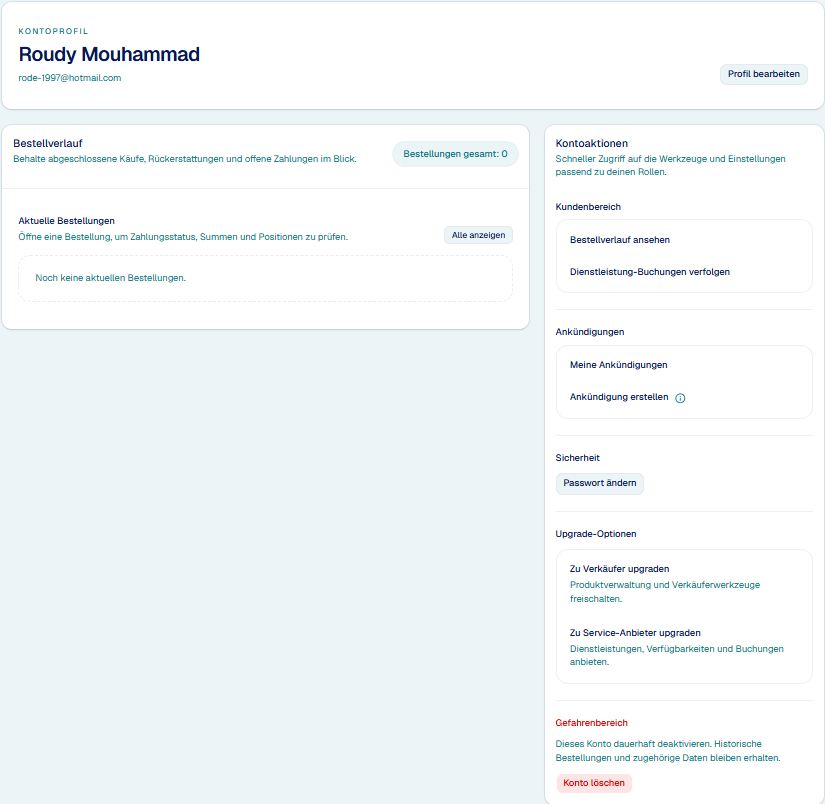
\includegraphics[width=0.85\textwidth]{Bilder/screenshot_kontoseite_kunde.png}
\caption{Kontoseite eines Nutzers ohne zusätzliche Rollen}
\label{fig:kontoseite_kunde}
\end{figure}
 
Für einen Nutzer ohne zusätzliche Rollen zeigt die rechte Spalte
allein den Kundenbereich, gefolgt von den rollenunabhängigen
Funktionen und den Anträgen auf ein Rollen-Upgrade. Die linke Spalte
enthält die eigene Bestellhistorie mit Datum, Betrag, Anzahl der
Positionen und Zahlungsstatus.
 
\begin{figure}[H]
\centering
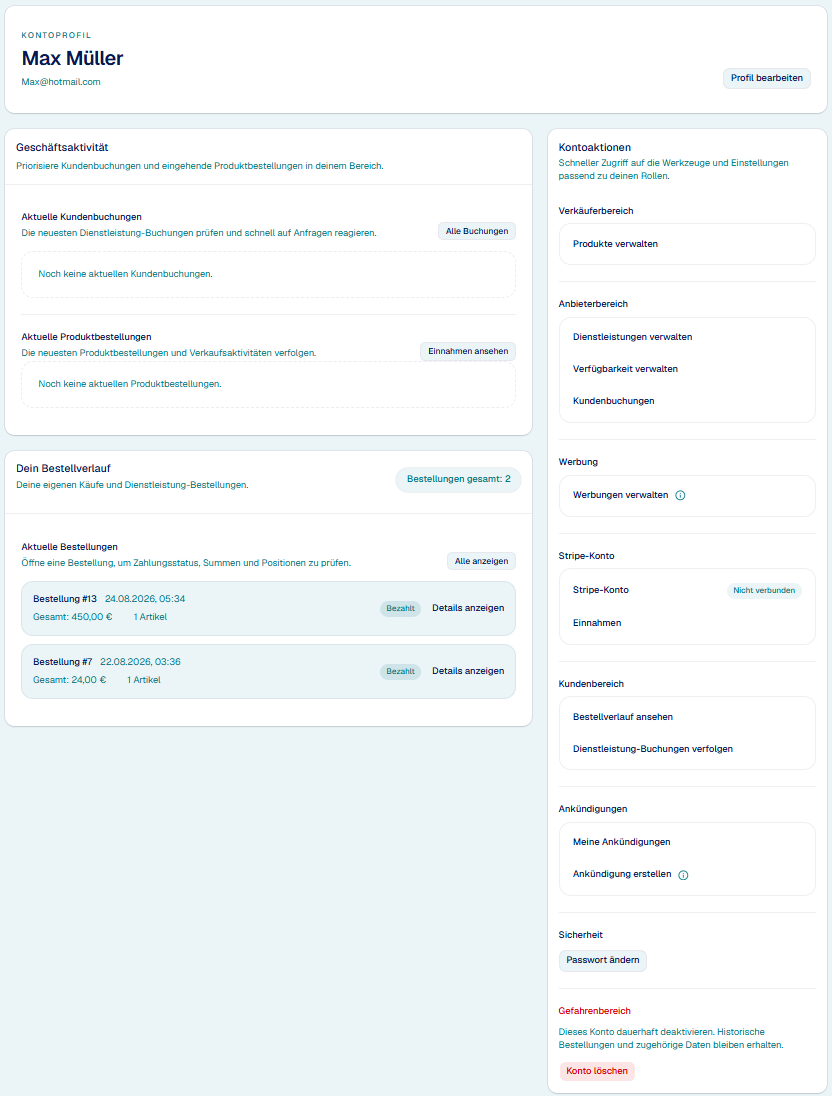
\includegraphics[width=0.85\textwidth]{Bilder/screenshot_kontoseite_anbieter.png}
\caption{Kontoseite eines Nutzers mit den Rollen 	extit{Seller} und
	extit{ServiceProvider}}
\label{fig:kontoseite_anbieter}
\end{figure}
 
Dieselbe Seite zeigt für einen Nutzer mit beiden anbietenden Rollen
drei Arbeitsbereiche untereinander: den Verkäuferbereich mit der
Produktverwaltung, den Anbieterbereich mit Dienstleistungen,
Verfügbarkeit und eingegangenen Buchungen sowie darunter den
Kundenbereich, den er als jeder andere Nutzer ebenfalls besitzt.
Anbindung an den Zahlungsdienst und Einnahmenübersicht erscheinen in
beiden anbietenden Bereichen, da sie für beide Rollen gelten.
 
Die Anträge auf ein Rollen-Upgrade entfallen hier vollständig. Sie
werden nur dann gerendert, wenn das Backend die jeweilige Rolle als
noch verfügbar meldet. Damit zeigt die Oberfläche keine Handlung an,
die für diesen Nutzer keine Wirkung mehr hätte.
 
Auch die linke Spalte wechselt mit der Rolle. Statt der eigenen
Bestellhistorie erscheint bei anbietenden Nutzern die
Geschäftsaktivität mit den eingegangenen Buchungen und
Produktbestellungen; die eigene Bestellhistorie wird darunter
zusätzlich eingeblendet, sofern eigene Bestellungen vorliegen.
Liegen für einen Bereich keine Einträge vor, erscheint an dessen
Stelle ein Hinweis statt einer leeren Fläche, wie er auch auf den
Katalogseiten verwendet wird (vgl.
Abschnitt~\ref{subsec:impl_produktlisting}).
 
Sämtliche Einträge der rechten Spalte werden über dieselbe
wiederverwendbare Komponente dargestellt, die Titel, Beschreibung,
Ziel und optional eine Zustandsmarkierung entgegennimmt. Aufbau und
Verhalten aller Einträge sind dadurch nicht durch Sorgfalt bei der
Umsetzung gleich, sondern durch Konstruktion. Die
Zustandsmarkierung wird bislang nur beim Zahlungsdienst verwendet
und zeigt dort an, ob das verbundene Konto eingerichtet ist. Ihre
Daten stammen aus einer eigenen Anfrage, die ausschließlich für
anbietende Nutzer ausgeführt wird.

\subsection{Dienstleistungsverwaltung: Zeitfenster und Abdeckungsbereich}
\label{subsec:impl_dienstleistungsverwaltung}
 
Dieser Abschnitt beschreibt sowohl die Verwaltung einzelner
Dienstleistungsangebote als auch die Verwaltung der Verfügbarkeit, die
als eigener Funktionsbereich \texttt{provider-availability/} umgesetzt
ist und derselben internen Struktur wie die übrigen Funktionsbereiche
folgt (vgl. Abschnitt~\ref{subsec:komponentenarchitektur}).
 
Die eigenen Dienstleistungen werden über \texttt{useMyServicesQuery}
abgerufen und seitenweise dargestellt; Seite und Ergebnisse pro Seite
sind, wie bereits beim Produktlisting beschrieben (vgl.
Abschnitt~\ref{subsec:impl_produktlisting}), Teil des Query Keys. Jede
Dienstleistung erscheint als Karte mit Kategorie, Preis, Dauer und
Veröffentlichungsstatus; gegenüber der öffentlichen Katalogansicht
ergänzt die Verwaltungskarte die Aktionen zum Ansehen, Bearbeiten und
Löschen.
 
\begin{figure}[H]
\centering
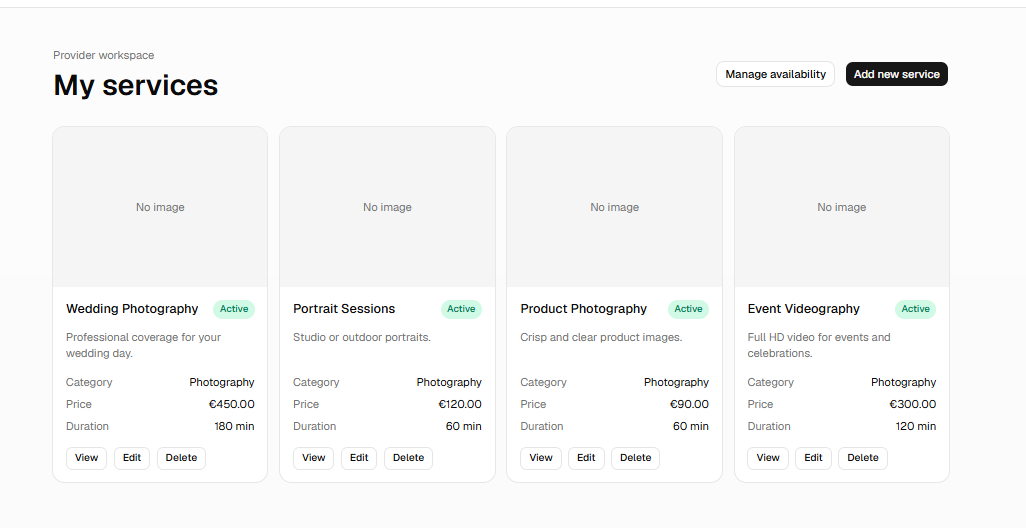
\includegraphics[width=\textwidth]{Bilder/screenshot_my_services.png}
\caption{Übersicht der eigenen Dienstleistungen mit den Aktionen zum Ansehen, Bearbeiten und Löschen}
\label{fig:my_services}
\end{figure}
 
Das Löschen einer Dienstleistung folgt demselben Muster wie die
Nebenwirkungen der Erfolgsseite (vgl.
Listing~\ref{lst:checkout-success}), betrifft jedoch vier
Zwischenspeicher zugleich: die eigene Übersicht, den öffentlichen
Dienstleistungskatalog, die zugehörige Detailseite und die
Startseite. Aus allen vieren muss der Eintrag zugleich verschwinden,
weshalb sie gezielt invalidiert werden, anstatt sich auf ein
automatisches Ablaufen zu verlassen (vgl.
Abschnitt~\ref{subsec:impl_tanstackquery}). Auf dem Bildschirm ist
davon nichts zu erkennen; sichtbar würde erst das Gegenteil, nämlich
eine Liste, in der ein bereits gelöschter Eintrag noch erscheint.
 
Beim Anlegen und Bearbeiten einer Dienstleistung werden neben Titel
und Beschreibung, die jeweils auf Englisch und Arabisch erfasst
werden, zugleich die Regeln für deren spätere Buchung festgelegt.
 
\begin{figure}[H]
\centering
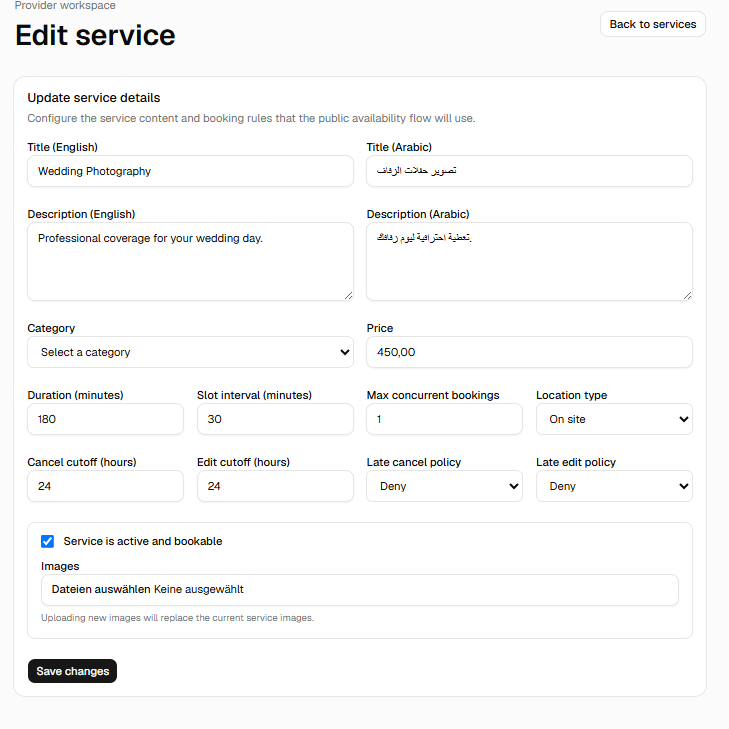
\includegraphics[width=\textwidth]{Bilder/screenshot_edit_service.png}
\caption{Formular zum Bearbeiten einer Dienstleistung mit
zweisprachigen Inhaltsfeldern und Buchungsregeln}
\label{fig:edit_service}
\end{figure}
 
Diese Regeln bestimmen, welche Termine die Buchungsansicht später
anbietet: Die Dauer legt die Länge eines Termins fest, das Zeitraster
den Abstand zwischen zwei möglichen Startzeitpunkten, und die maximale
Anzahl gleichzeitiger Buchungen bestimmt, wie viele Kunden denselben
Zeitraum belegen können. Hinzu kommen der Ort der Leistungserbringung
sowie getrennte Fristen für Stornierung und Änderung, jeweils mit der
Festlegung, wie nach Ablauf der Frist zu verfahren ist.
 
Die Verfügbarkeit wird davon getrennt verwaltet, da sie nicht für eine
einzelne Dienstleistung, sondern für alle Angebote eines Anbieters
gemeinsam gilt.
 
\begin{figure}[H]
\centering
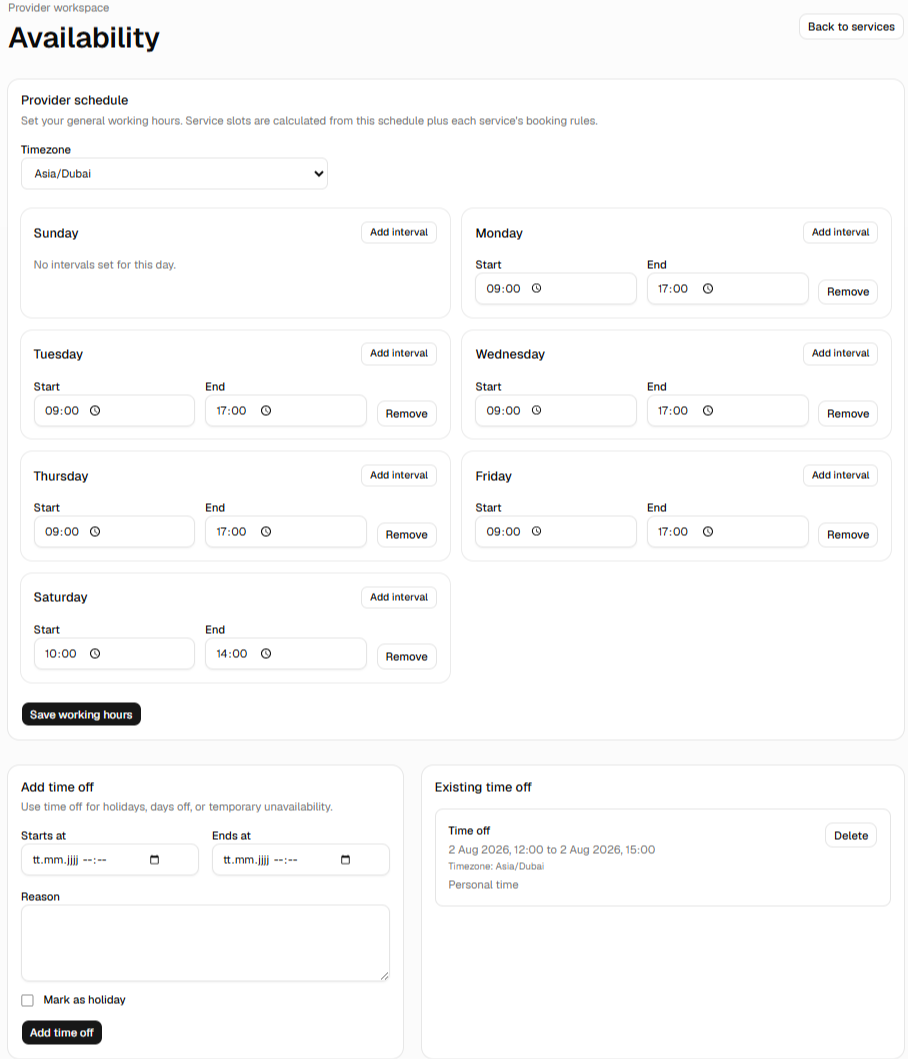
\includegraphics[width=0.7\textwidth]{Bilder/screenshot_availability.png}
\caption{Verfügbarkeitsverwaltung mit Wochenschema und einzelnen Abwesenheitszeiträumen}
\label{fig:availability}
\end{figure}
 
Die festen Arbeitszeiten werden je Wochentag über die
wiederverwendbare Komponente \texttt{WorkingHoursEditor} dargestellt,
die für jeden Wochentag beliebig viele Zeitintervalle mit Start- und
Endzeit entgegennimmt und es erlaubt, einzelne Intervalle hinzuzufügen
oder zu entfernen. Ein Wochentag ohne Intervall gilt als nicht
verfügbar.
 
Das Formular \texttt{TimeOffForm} für einzelne Abwesenheitszeiträume
ist als eigene Komponente ausgelagert, da es an mehreren Stellen
innerhalb des Funktionsbereichs wiederverwendet wird. Seine Eingaben
werden über ein Zod-Schema validiert (vgl.
Abschnitt~\ref{subsec:formulare-validierung}), das bewusst mit den
Validierungsregeln des Backends übereinstimmt, sodass ein Nutzer, der
die Formularvalidierung durch direkte Manipulation der
Benutzeroberfläche umgeht, spätestens bei der serverseitigen Prüfung
denselben Regeln unterliegt.
 
Der Abruf der Verfügbarkeitsdaten erfolgt über
\texttt{useProviderAvailabilityQuery}, das Hinzufügen eines
Abwesenheitszeitraums über eine Mutation, die den zugehörigen
Cache-Eintrag im Erfolgsfall invalidiert, sodass die Liste automatisch
aktualisiert wird. Die eingetragenen Zeiträume werden nach ihrem
Beginn sortiert angezeigt und anhand der beim Anbieter hinterlegten
Zeitzone formatiert, nicht anhand der Zeitzone des aufrufenden
Endgeräts, damit Kunden die Verfügbarkeit unabhängig vom eigenen
Standort korrekt einschätzen können.
\subsection{Produktverwaltung}
\label{subsec:impl_produktverwaltung}

Die Produktverwaltung folgt strukturell demselben Muster wie die
in Abschnitt~\ref{subsec:impl_dienstleistungsverwaltung}
beschriebene Dienstleistungsverwaltung, ist jedoch einfacher, da
Produkte im Gegensatz zu Dienstleistungen keine Buchungsregeln
benötigen.

% TODO (Roudy): Hier kommt der Screenshot von "My products"
% hin (Kartenuebersicht der eigenen Produkte).

Die eigenen Produkte werden über \texttt{useMyProductsQuery}
abgerufen und nach demselben Kartenprinzip dargestellt, das auch
auf der öffentlichen Katalogseite zum Einsatz kommt (vgl.
Abschnitt~\ref{subsec:impl_produktlisting}); die
Verwaltungskarte ergänzt dabei Aktionen zum Bearbeiten
und Löschen. Das Löschen eines Produkts verfährt ebenso, betrifft aber nur drei
Zwischenspeicher, da eine eigene Detailseite im Zwischenspeicher
nicht gesondert geführt wird: die eigene Produktliste, den
öffentlichen Katalog und die Produkte des Verkäuferprofils.

% TODO (Roudy): Hier kommt der Screenshot vom "Edit product"-
% Formular hin.

Die erfassten Felder entsprechen dabei denen der
Dienstleistungsverwaltung, abzüglich der dort beschriebenen
Buchungsregeln (vgl.
Abschnitt~\ref{subsec:verkaeufer_dashboard_konzept}).


\subsection{Eingegangene Buchungen}
\label{subsec:impl_provider_bookings}
Die Ansicht der eingegangenen Buchungen setzt die in
Abschnitt~\ref{subsec:verkaeufer_dashboard_konzept} beschriebene
Zustandsfolge um. Jede Buchung erscheint als Eintrag mit Kunde,
Beginn, Ende und Zeitzone sowie einer Zustandsmarkierung.
 
\begin{figure}[H]
\centering
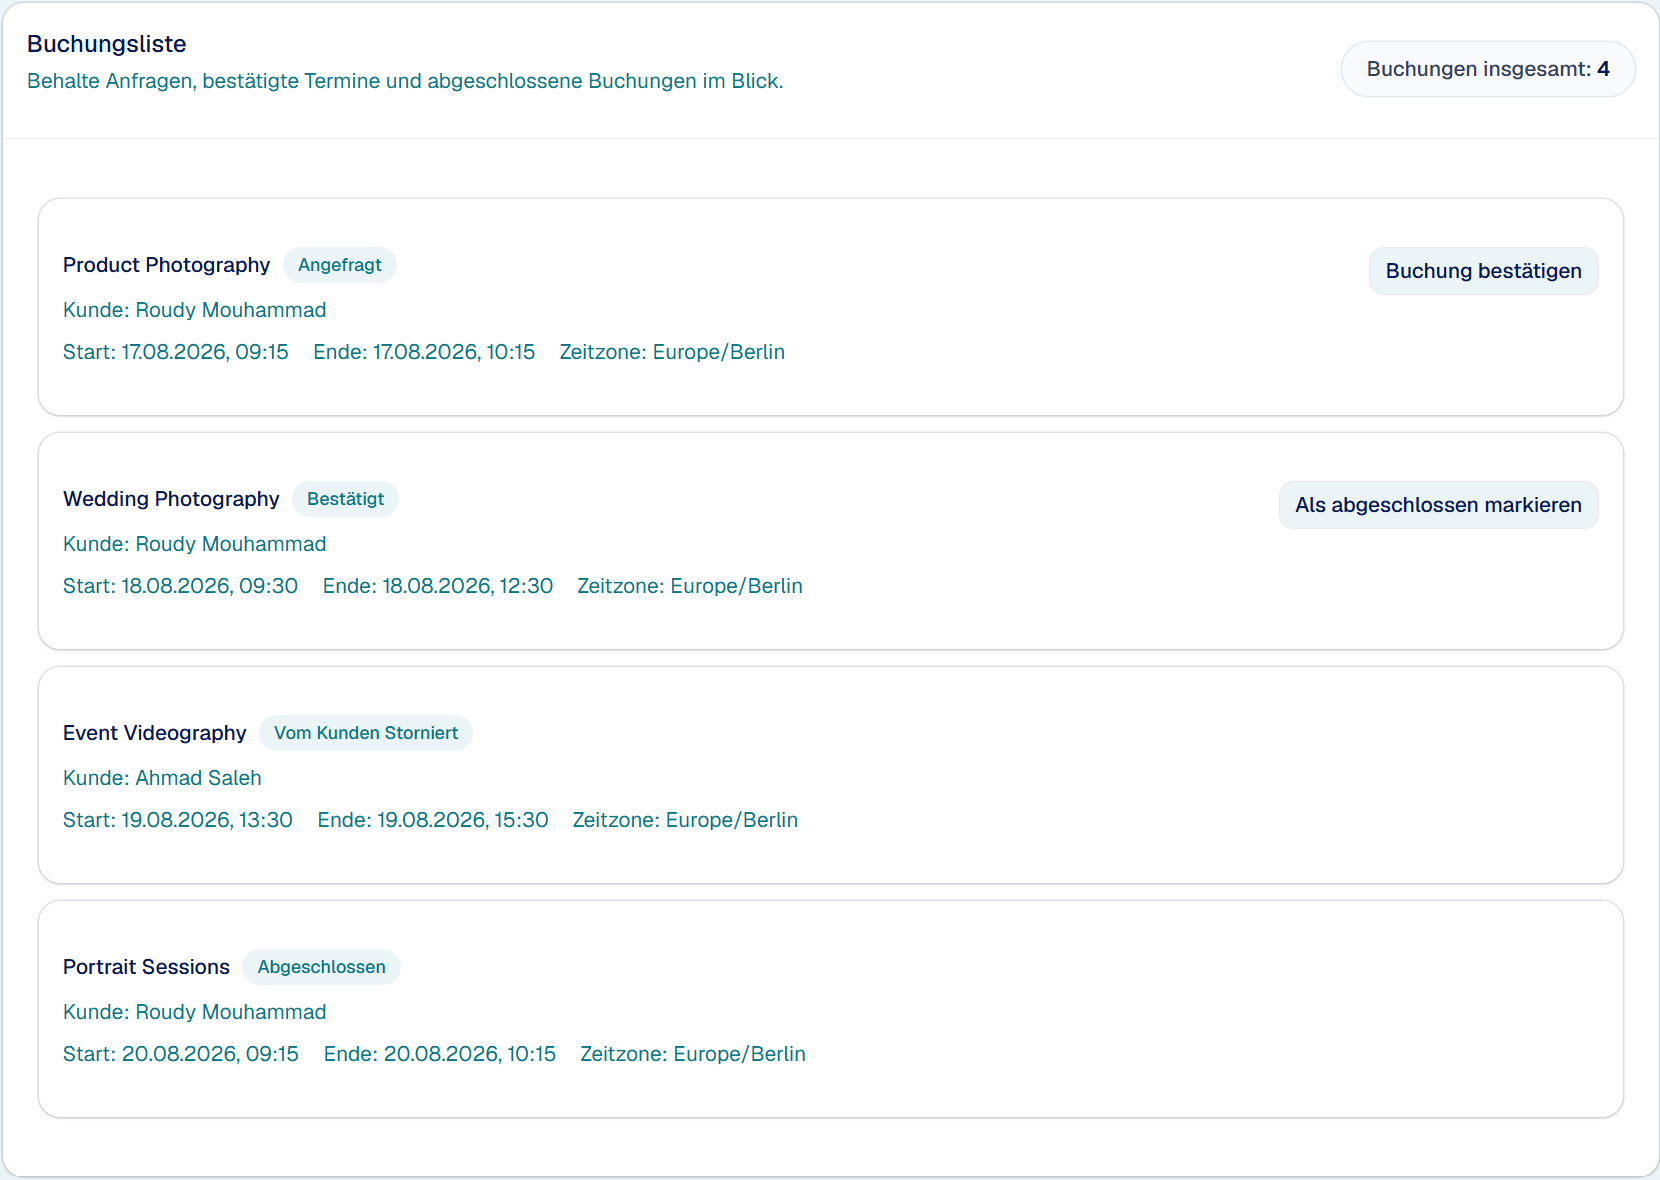
\includegraphics[width=\textwidth]{Bilder/screenshot_provider_bookings.png}
\caption{Eingegangene Buchungen mit der jeweils zustandsabhängigen
Aktion}
\label{fig:provider_bookings}
\end{figure}
 
Rechts neben jedem Eintrag steht genau eine Schaltfläche, und welche
das ist, ergibt sich aus dem Zustand: Bei einer angefragten Buchung
lautet sie \textit{Buchung bestätigen}, bei einer bereits bestätigten
\textit{Als abgeschlossen markieren}. Eine abgeschlossene Buchung
trägt keine Schaltfläche mehr. Die Oberfläche zeigt damit nicht alle
denkbaren Aktionen mit wechselnder Verfügbarkeit, sondern jeweils nur
die eine, die im gegenwärtigen Zustand möglich ist.
 
Beide Übergänge sind als Mutationen umgesetzt, die den
zwischengespeicherten Bestand der Buchungsliste im Erfolgsfall
invalidieren (vgl. Abschnitt~\ref{subsec:impl_tanstackquery}), sodass
der neue Zustand unmittelbar erscheint, ohne dass die Seite neu
geladen werden muss.


\subsection{Bestellhistorie und Bestelldetail}
\label{subsec:impl_bestellungen}

Die Bestellübersicht führt sämtliche Aufträge des Nutzers mit Datum,
Gesamtbetrag, Anzahl der Positionen und Zahlungsstatus. Der Aufruf
eines Eintrags führt auf die Detailseite, die den Auftrag in zwei
Bereiche gliedert: eine Zusammenfassung mit den Kopfdaten und die
Liste der enthaltenen Positionen.
 
Da ein Auftrag bereits vor der Zahlung entsteht (vgl.
Abschnitt~\ref{subsec:warenkorb_konzept}), unterscheidet die
Detailseite zwei Fälle. Bei einem unbezahlten Auftrag tritt an die
Stelle der Positionsliste ein eigener Bereich, der den Zustand
benennt und zwei Wege anbietet.
 
\begin{figure}[H]
\centering
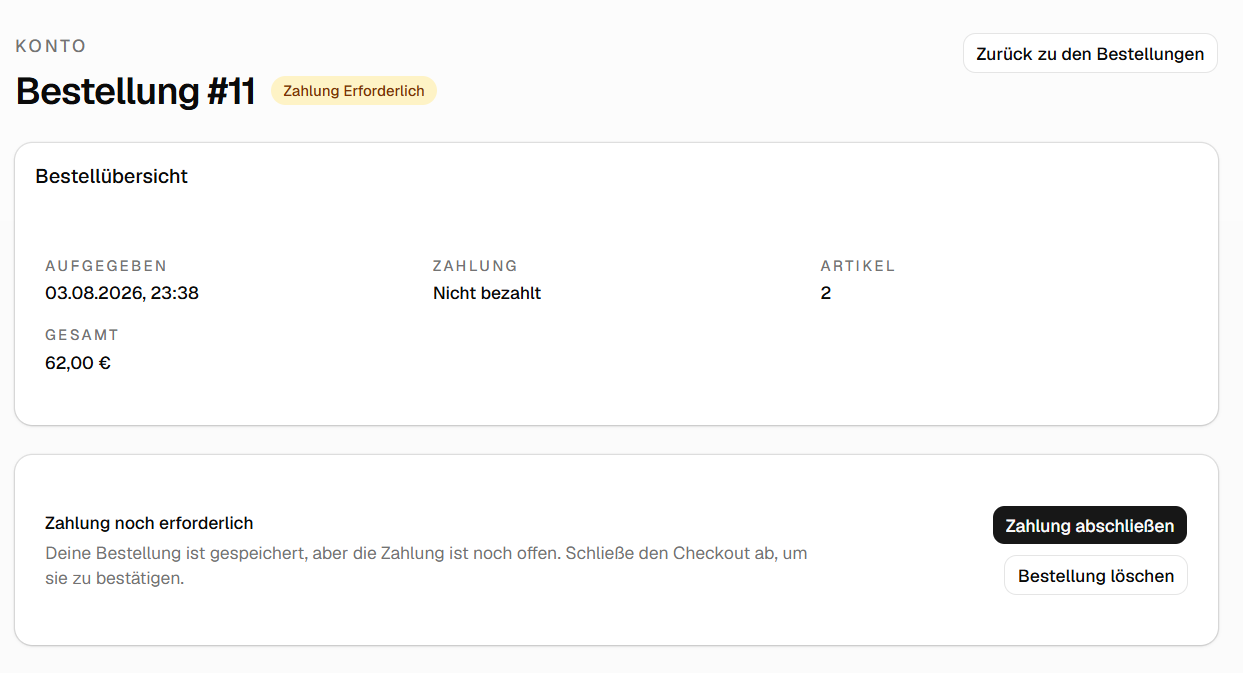
\includegraphics[width=\textwidth]{Bilder/screenshot_bestellung_unbezahlt.png}
\caption{Detailansicht eines Auftrags, dessen Zahlung nicht
abgeschlossen wurde}
\label{fig:bestellung_unbezahlt}
\end{figure}
 
Verlässt ein Nutzer die Zahlungsseite, ohne den Vorgang
abzuschließen, bleibt der Auftrag in diesem Zustand bestehen. Er
lässt sich entweder nachträglich bezahlen oder verwerfen. Ohne diese
beiden Möglichkeiten entstünde bei jedem abgebrochenen
Zahlungsvorgang ein Eintrag, den der Nutzer weder abschließen noch
entfernen könnte. Der Fall betrifft Produkte und
Dienstleistungsbuchungen gleichermaßen.
 
Bei einem bezahlten Auftrag erscheint dagegen die vollständige
Positionsliste. Jede Position trägt ihren eigenen Zustand, da
Produkte und Dienstleistungen unabhängig voneinander bearbeitet
werden.
 
\begin{figure}[H]
\centering
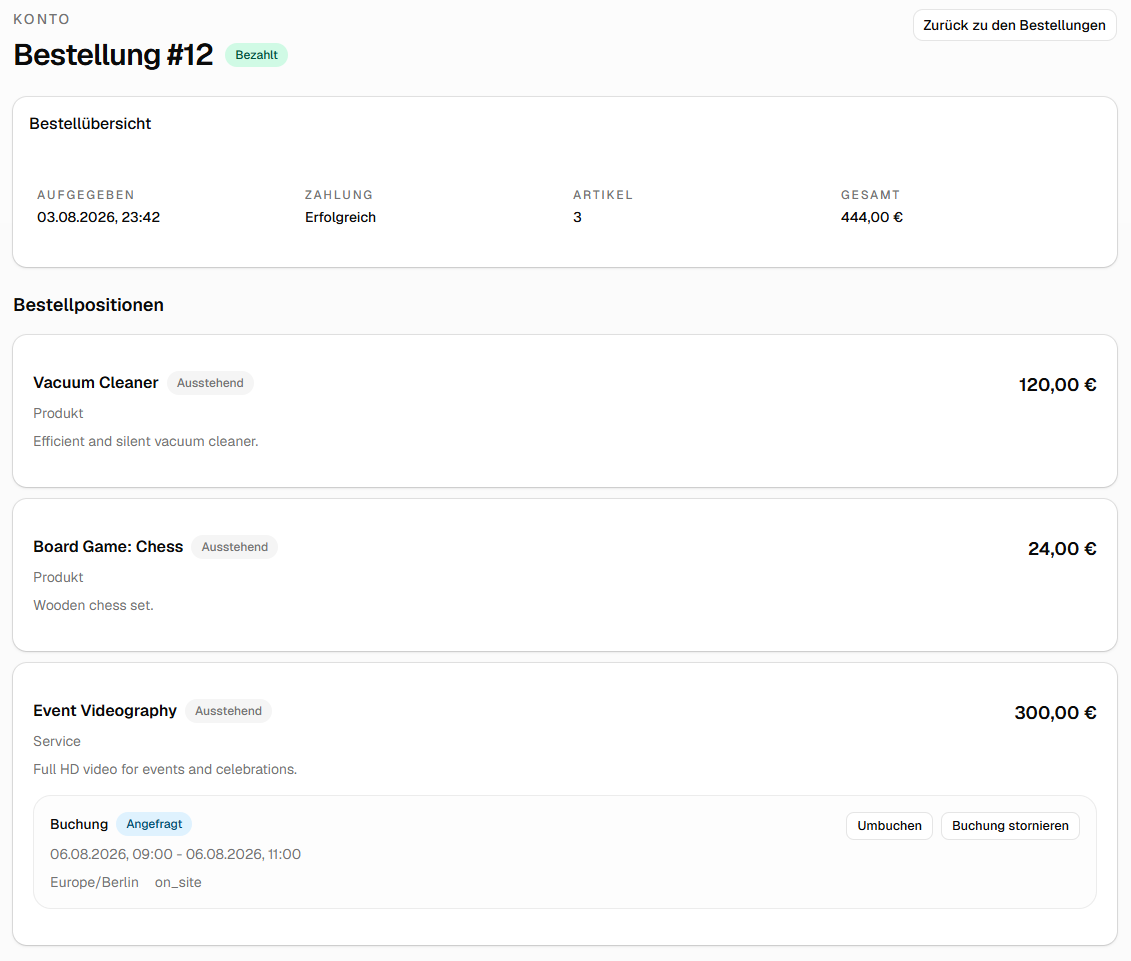
\includegraphics[width=0.85\textwidth]{Bilder/screenshot_bestelldetail.png}
\caption{Detailansicht eines bezahlten Auftrags mit Produkt- und
Dienstleistungspositionen}
\label{fig:bestelldetail}
\end{figure}
 
Eine Dienstleistungsposition führt dabei die zugehörige Buchung mit:
Termin, Zeitzone und Ort der Leistungserbringung erscheinen innerhalb
der Position, zusammen mit den Schaltflächen zum Umbuchen und
Stornieren. Dieselben Aktionen sind auch über die Buchungsübersicht
erreichbar (vgl. Abschnitt~\ref{subsec:impl_buchungen}). Die
doppelte Erreichbarkeit ist beabsichtigt: Ein Nutzer, der von einer
Bestellung ausgeht, soll die zugehörige Buchung nicht in einer
anderen Ansicht suchen müssen.

\subsection{Buchungsübersicht, Stornierung und Umbuchung}
\label{subsec:impl_buchungen}

Die Buchungsübersicht führt die gebuchten Termine des Nutzers mit
Dienstleistung, Anbieter, Zeitraum, Zeitzone, Ort und Zustand. Unter
jedem Eintrag stehen zwei Blöcke, einer für die Stornierung und einer
für die Umbuchung, in denen die beim Anlegen der Dienstleistung
festgelegten Fristen wiedergegeben werden (vgl.
Abschnitt~\ref{subsec:impl_dienstleistungsverwaltung}). Solange eine
Frist läuft, nennt der zugehörige Block den Zeitpunkt ihres Endes,
und die Schaltfläche ist auslösbar.
 
\begin{figure}[H]
\centering

\includegraphics[width=\textwidth]{Bilder/screenshot_buchung_offen.png}
\caption{Buchung innerhalb der Fristen: beide Aktionen verfügbar,
jeweils mit Angabe des Fristendes}
\label{fig:buchung_offen}
\end{figure}
 
Nach Ablauf einer Frist wird die zugehörige Schaltfläche deaktiviert,
und an die Stelle des Fristendes tritt der Hinweis, dass der Zeitraum
verstrichen ist. Beide Schaltflächen bleiben dabei sichtbar --
dieselbe Entscheidung wie bei der Terminauswahl, in der ein nicht
verfügbarer Tag benannt statt ausgeblendet wird (vgl.
Abschnitt~\ref{subsec:impl_terminauswahl}).
 
\begin{figure}[H]
\centering

\includegraphics[width=\textwidth]{Bilder/screenshot_buchung_frist_abgelaufen.png}
\caption{Buchung nach Ablauf beider Fristen: die Schaltflächen sind
deaktiviert, der Grund steht darüber}
\label{fig:buchung_frist_abgelaufen}
\end{figure}
 
Die Umbuchung führt auf eine eigene Seite, die dieselbe
Terminauswahl verwendet wie die Erstbuchung. Die Komponente ist damit
an zwei Stellen der Anwendung eingesetzt, ohne dass die Ermittlung
verfügbarer Zeitfenster ein zweites Mal umgesetzt werden musste.
Neben der Auswahl zeigt die Seite den bisherigen Termin, sodass der
Wechsel nachvollziehbar bleibt.
 
Eine Stornierung löst dagegen keine erneute Auswahl aus, sondern eine
Rückerstattung über das Backend, deren Stand anschließend an der
Buchung selbst geführt wird.

% ----------------------------------------------------------------

\section{Werbung und Ankündigungen}
\label{sec:impl_werbung}

% TODO: Implementierung der Ankündigungen und Werbemodule je Rolle,
% Genehmigungsprozess.

% ----------------------------------------------------------------
\section{Messaging}
\label{sec:impl_messaging}
Die Umsetzung des in Abschnitt~\ref{subsec:messaging_konzept}
beschriebenen Nachrichtenbereichs besteht aus zwei Teilen, die
unabhängig voneinander arbeiten: dem gewöhnlichen, anfragebasierten
Zugriff auf Unterhaltungen und Nachrichten und der Anbindung an den
Echtzeitdienst. Der erste Teil folgt dem in
Abschnitt~\ref{subsec:impl_featureapi} beschriebenen Aufbau und
verwendet dieselbe \acs{HTTP}-Instanz wie alle übrigen
Funktionsbereiche; er liefert die Liste der Unterhaltungen, den
Verlauf einer Unterhaltung und den Zählerstand ungelesener
Nachrichten und nimmt gesendete Nachrichten entgegen. Der zweite
Teil ist Gegenstand dieses Abschnitts.
 
 
\subsection{Anbindung des Echtzeitdienstes}
\label{subsec:impl_pusher_client}
 
Die Verbindung wird in einem eigenen Modul gekapselt, das als
einzige Stelle der Anwendung die Bibliothek des Dienstanbieters
kennt. Es hält die Verbindung in einer Modulvariablen und gibt eine
bereits bestehende Verbindung zurück, statt eine zweite aufzubauen.
Diese Festlegung ist notwendig, weil mehrere Stellen der Anwendung
unabhängig voneinander Kanäle abonnieren: die Chatseite für jede
Unterhaltung und die Kopfzeile für den Zählerstand. Ohne die
Bündelung entstünde je Aufruf eine eigene Verbindung.
 
\begin{lstlisting}[language=TypeScript,caption={Aufbau der Verbindung
zum Echtzeitdienst},label={lst:pusher-client}]
let client: Pusher | null = null
 
export function getPusherClient() {
  const token = getAuthToken()
  const config = getPusherConfig()
 
  if (!token || !config) {
    return null
  }
 
  if (client) {
    return client
  }
 
  client = new Pusher(config.key, {
    cluster: config.cluster,
    authEndpoint: getBroadcastAuthEndpoint(),
    auth: {
      headers: { Authorization: `Bearer ${token}` },
    },
  })
 
  return client
}
\end{lstlisting}
 
Drei Angaben bestimmen die Verbindung. Der Schlüssel identifiziert
das Projekt beim Dienstanbieter. Der \emph{Cluster} benennt die
Region, in der die Kanäle betrieben werden, und ist damit für die
Laufzeit einer Nachricht maßgeblich. Der dritte Wert ist die
Adresse, an die der Dienst seine Freigabeanfragen richtet: Meldet
sich der Client für einen privaten Kanal an, fragt die Bibliothek
zunächst beim Backend nach, ob er dazu berechtigt ist. Da diese
Anfrage nicht über die zentrale \acs{HTTP}-Instanz aus
Abschnitt~\ref{subsec:impl_httpclient} läuft, sondern von der
Bibliothek selbst gestellt wird, muss der Authentifizierungstoken
hier ein zweites Mal ausdrücklich mitgegeben werden.
 
Ohne angemeldeten Nutzer liefert die Funktion keinen Client. Der
Nachrichtenbereich ist damit auch technisch an die Anmeldung
gebunden und nicht allein über den Routenschutz aus
Abschnitt~\ref{subsec:impl_token_session}.
 
 
\subsection{Nachrichtenoberfläche}
\label{subsec:impl_chat_ui}
 
Die Chatseite ist zweispaltig aufgebaut. Links steht die Liste der
Unterhaltungen mit Name des Gegenübers, Zeitpunkt und Anfang der
letzten Nachricht, rechts der Verlauf der ausgewählten Unterhaltung.
Die gewählte Unterhaltung steht als Bestandteil der Adresse
(\texttt{/chat/:conversationId}), sodass eine einzelne Unterhaltung
verlinkbar bleibt -- dieselbe Entscheidung wie bei den Katalogseiten,
auf denen Seite und Kategorie ebenfalls in der Adresse stehen (vgl.
Abschnitt~\ref{subsec:impl_produktlisting}).
Ist keine Unterhaltung angegeben, wird auf die zuletzt aktive
umgeleitet.
 
\begin{figure}[H]
\centering
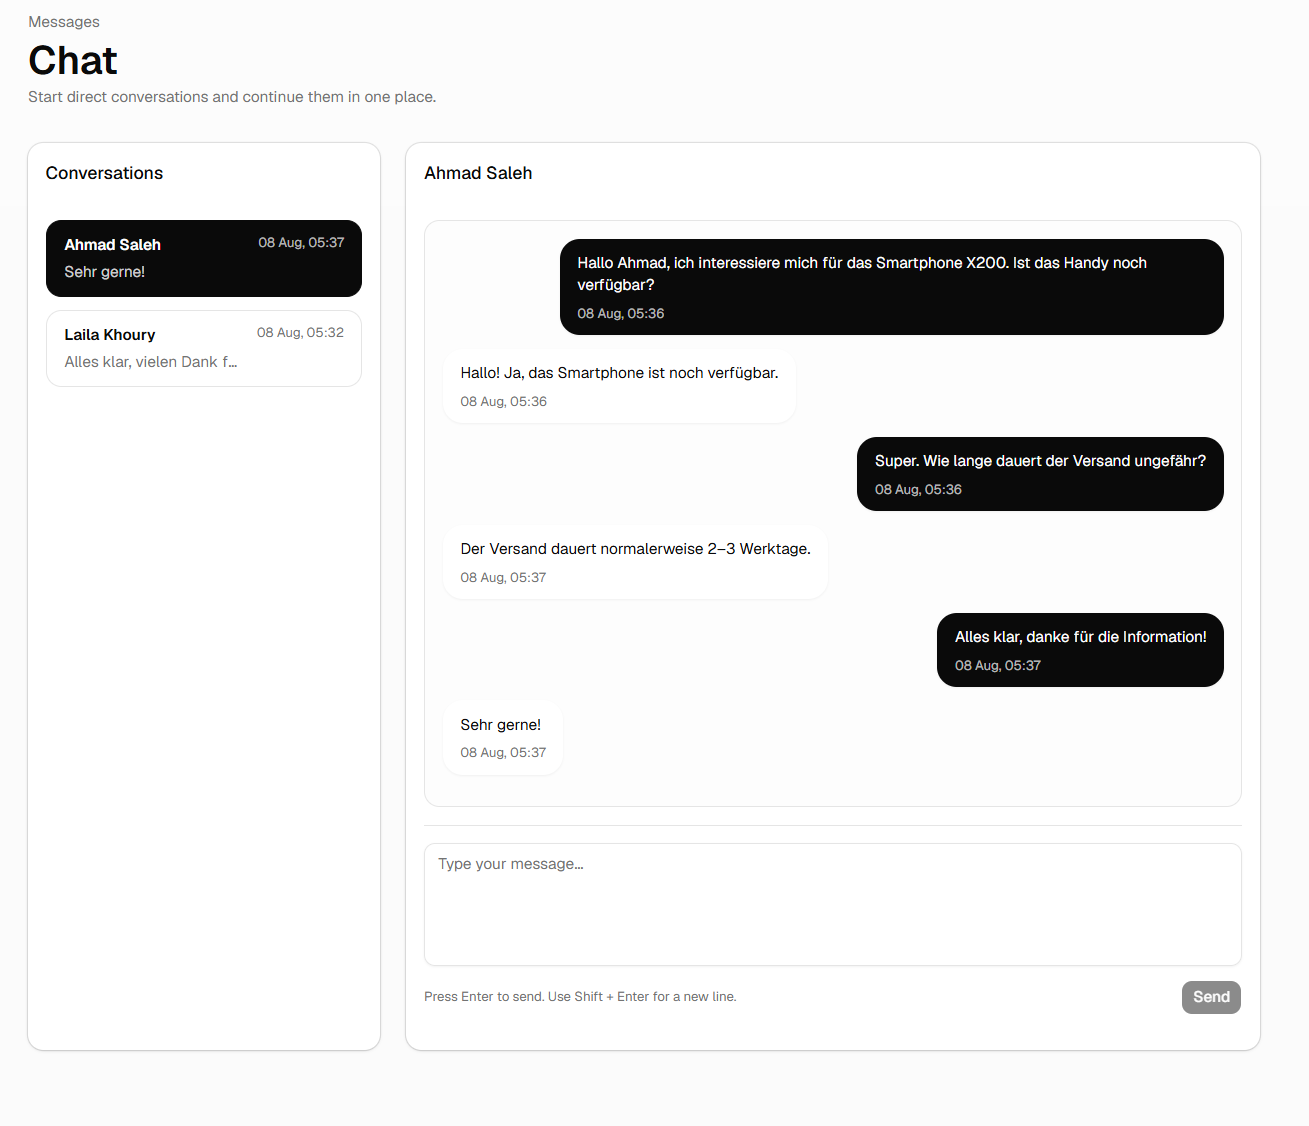
\includegraphics[width=\textwidth]{Bilder/screenshot_chat.png}
\caption{Nachrichtenbereich mit Liste der Unterhaltungen und
Verlauf}
\label{fig:chat_seite}
\end{figure}
 
Eigene und empfangene Nachrichten unterscheiden sich in Ausrichtung
und Farbe. Die Zuordnung erfolgt nicht über die Reihenfolge, sondern
über den Vergleich der Absenderkennung mit der Kennung des
angemeldeten Nutzers -- eine Nachricht, die über den Kanal
eintrifft, trägt dieselbe Struktur wie eine aus der Datenbank
geladene und wird deshalb gleich behandelt.
 
Die Unterhaltungen werden nach dem Zeitpunkt der letzten Nachricht
sortiert, sodass die zuletzt genutzte oben steht. Da diese
Sortierung sowohl beim Laden als auch beim Eintreffen einer
Nachricht über den Kanal angewendet werden muss, ist sie als eigene
Funktion ausgelagert.
 
 
\subsection{Abonnement der Kanäle und Aktualisierung des
Zwischenspeichers}
\label{subsec:impl_chat_realtime}
 
Sobald die Liste der Unterhaltungen vorliegt, meldet sich die Seite
für jede darin enthaltene Unterhaltung beim zugehörigen Kanal an.
Die Kanalnamen ergeben sich unmittelbar aus der Kennung der
Unterhaltung, sodass keine gesonderte Zuordnung geführt werden muss.
Auf jedem Kanal werden drei Ereignisse ausgewertet: das Eintreffen
einer Nachricht sowie die Bestätigung ihrer Zustellung und ihres
Lesens.
 
Entscheidend ist, was beim Eintreffen eines Ereignisses geschieht.
Die Anwendung stellt keine neue Anfrage an das Backend, sondern
schreibt die empfangene Nachricht unmittelbar in den
Zwischenspeicher von TanStack Query (vgl.
Abschnitt~\ref{subsec:impl_tanstackquery}). Eine erneute Anfrage wäre
überflüssig, da die Nachricht bereits vollständig vorliegt; sie
würde die Ersparnis, die die dauerhafte Verbindung gerade bewirkt,
wieder aufheben.
 
\begin{lstlisting}[language=TypeScript,caption={Eintragen einer über
den Kanal empfangenen Nachricht in den Zwischenspeicher},
label={lst:chat-cache}]
queryClient.setQueryData<ChatMessagesResponse | undefined>(
  ['chat', 'messages', conversationId],
  (currentData) => {
    if (!currentData?.result) {
      return currentData
    }
 
    if (currentData.result.data.some((m) => m.id === normalizedMessage.id)) {
      return currentData
    }
 
    return {
      ...currentData,
      result: {
        ...currentData.result,
        data: [...currentData.result.data, normalizedMessage],
        total: currentData.result.total + 1,
      },
    }
  },
)
\end{lstlisting}
 
Die Prüfung auf eine bereits vorhandene Kennung ist erforderlich,
weil der Absender seine eigene Nachricht auf zwei Wegen erhält:
einmal als Antwort auf die absendende Anfrage und einmal über den
Kanal, auf dem sie veröffentlicht wird. Ohne diese Prüfung erschiene
sie doppelt.
 
Parallel dazu wird die Liste der Unterhaltungen fortgeschrieben:
Vorschautext und Zeitpunkt der betroffenen Unterhaltung werden
ersetzt, die Liste neu sortiert und der Zähler ungelesener
Nachrichten erhöht -- letzteres nur dann, wenn die Nachricht nicht
vom Nutzer selbst stammt und die betroffene Unterhaltung nicht gerade
geöffnet ist.
 
Die Anmeldung an den Kanälen erfolgt in einem Effekt, dessen
Aufräumfunktion die Ereignisbindungen löst und die Kanäle wieder
abmeldet. Unterbleibt dies, laufen nach einem Wechsel der Seite
weiterhin Ereignisse in Funktionen, die auf einen nicht mehr
dargestellten Zustand zugreifen; zugleich blieben die Kanäle
abonniert und die Zahl der Abonnements stiege mit jedem Aufruf der
Seite. Aus demselben Grund wird die Liste der Unterhaltungen mit
\texttt{useMemo} stabil gehalten: Entstünde bei jedem Rendern ein
neues Feld, liefe der Effekt jedes Mal erneut und meldete sämtliche
Kanäle ab und wieder an.
 
Der Zähler ungelesener Nachrichten in der Kopfzeile ist in einem
eigenen Hook gekapselt, der den auf den Nutzer bezogenen Kanal
abonniert und den empfangenen Gesamtstand in denselben
Zwischenspeicher schreibt, aus dem die Anzeige liest. Er ist
unabhängig von der Chatseite und damit in der gesamten Anwendung
wirksam.
 
Wird eine Unterhaltung geöffnet, prüft die Seite, ob sie ungelesene
Nachrichten des Gegenübers enthält, meldet sie gegebenenfalls als
gelesen und setzt den Zähler der betroffenen Unterhaltung
anschließend lokal auf null, ohne die Liste erneut abzurufen.
